\section{Repaired Interaction Semantics}
\label{sec:overview-semantics}

We briefly review interaction semantics (\Cref{sec:overview-semantics:background}), discuss the problems (\Cref{sec:overview-semantics:problems}) and present our solutions (\Cref{sec:overview-semantics:solution}).

\subsection{Background}
\label{sec:overview-semantics:background}

We give a brief overview of interaction semantics of \ccc{}, which
interactively executes modules equipped with their own independent
module semantics. Each module semantics $M$ provides
a set of module states (also called \emph{cores}) $\States{M}$ with the following operations:
\begin{itemize}
\item \texttt{init\_core}: given a function $f$ with arguments $\vec{v}$,
  %and a memory $m$,
  gives the initial module state $s \in \States{M}$
  % with updated memory $m'$
  executing the invoked function $f$ with $\vec{v}$.
\item \texttt{at\_external}: given $s \in \States{M}$,
  %and a memory $m$,
  checks if an external function $f$ is called with arguments~$\vec{v}$.
  %% and if so, gives updated memory $m'$ and state $s'$.
\item \texttt{after\_external}: given $s \in \States{M}$
  where an external function is called,
  %a memory $m$
  and a return value $r$,
  gives the module state $s'$
  %and memory $m'$
  after the function call returns $r$.
\item \texttt{halted}: given $s \in \States{M}$, checks if the module execution is halted with a return value~$r$.
\item \texttt{corestep}: given $s \in \States{M}$ and memory $m$, takes a local step producing an event $e$ and the next state~$s'$ with updated memory $m'$.
\end{itemize}

We explain how interaction semantics works using an example in
\Cref{fig:inter-sem}, where the whole machine state consists of a
memory, say $m$, and a stack of module states (called \emph{core stack}), say $[s_2; s_1]$.
Then, interaction semantics checks whether the stack-top module $s_2$
is invoking an external function using \texttt{at\_external}, and if
so, pushes the invoked module's initial state, say $s_3$, obtained by
\texttt{init\_core}. Note here that the same module $M_1$ can have
multiple module states $s_1$ and $s_3$ in the stack.  Then the
new top module $s_3$ takes a local step to $s_3'$ with updated memory
$m'$ according to its \texttt{corestep}, and if $s_3'$ is a halted
state with a return value $r$ (checked with \texttt{halted}), the top
module $s_3'$ is popped and returned to the next module $s_2$, which
is then updated to $s_2'$ given by \texttt{after\_external} with the return
value $r$.

\begin{figure}[t]
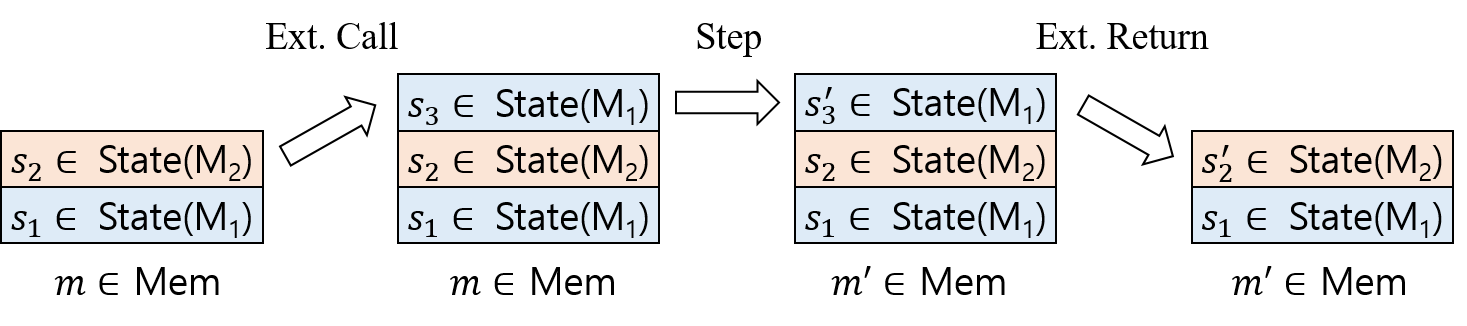
\includegraphics[width=0.9\linewidth]{images/intersem.png}
\caption{An execution of interaction semantics}
\label{fig:inter-sem}
\end{figure}

%% marshalling unmarshalling
%% marshalling the argument values into a list of values
%% setting the initial core states, unmarshalling the list of arguments.
%% at\_external: marshalling the argument values into a list of values
%% after\_external: unmarshalling the return value into
%% halted: marshalling the return value
%% corestep: use the underlying language semantics

Finally, note that the language semantics of C, assembly and
intermediate languages can be lifted to give a module semantics by
defining \texttt{corestep} to be the same as the execution step of the
language's semantics, and the other module operations to reflect the
calling conventions. Note also that all language-specific resources
(\ie other than the memory)
such as the register-file of assembly 
reside inside the module state, and thus are
duplicated at each invocation of a module.

%% One can lift a \cc{} language semantics into a core semantics by providing the interfaces:
%% Note that it is possible to define a core semantics using a mathematical specification.

\subsection{Problems}
\label{sec:overview-semantics:problems}

The problems with the interaction semantics of \ccc{} are that it does
not satisfy two adequacy properties. First, the adequacy w.r.t. C says
that for any C modules $M_1,\ldots,M_n$, the behaviors of the linked
program according to interaction semantics $\beh{M_1 \llink
  \ldots \llink M_n}$ should \emph{be included in} those according to the
physical semantics $\beh{M_1 \plink \ldots\plink M_n}$.  The reason for
failure was quite simple and we could easily fix it: unlike \ccc{}, we allow passing
the \texttt{undef} value to an external module since the C semantics
does so, while we turn ill-typed values into \texttt{undef} when they
are passed to an external module.

Second, the failure of the adequacy w.r.t. assembly is more serious.
Adequacy says that for any assembly modules $M_1,\ldots,M_n$,
the behaviors of the linked program according to interaction
semantics $\beh{M_1 \llink \ldots \llink M_n}$ should \emph{include}
those according to the physical semantics $\beh{M_1 \plink \ldots\plink M_n}$.
Note that the direction is opposite since assembly is the target language.
As discussed before, the reason for failure is that
the interaction semantics of \ccc{} does not have a mechanism to detect
illegal interference and make it undefined behavior~(UB).

%% A serious problem with the interaction semantics of \ccc{} is that it
%% is not correctly related to the physical assembly behavior. More
%% precisely, the behaviors of linked assembly modules according to
%% interaction semantics does not always include those according to \cc{}'s
%% assembly semantics, and in fact \ccc{} missed such a proof.

%% The problem is interference, which does not occur in the interaction
%% semantics due to logical isolation (ie, registers and argument area of
%% stack are not shared), but occurs in the physical behavior.

%% This problem, rather surprisingly, involves an essential and
%% challenging issue with linking with \emph{arbitrary} assembly
%% code. The issue is that arbitrary assembly code, unlike
%% compiler-generated assembly code, may break compilers' implicit
%% assumptions that their optimizations rely on.
%% \todo{make it clearer: Indeed \ccc{}'s
%% interaction semantics implicitly imposes such assumptions at
%% intermodule steps regardless of the actual behavior of assembly code.}
%% While this enables proving the optimizations correct, it makes the
%% interaction semantics deviate from the actual assembly semantics.
%%

\subsection{Our Solution}
\label{sec:overview-semantics:solution}

We identify the sources of inadequacy w.r.t. assembly as violations of
three assumptions made by standard compilers: two on the registers and one on the stack.
We discuss why they 
cause problems with counterexamples and show how to semantically
handle them without changing the underlying language semantics.

%% we figured out that there are three calling conventions that are the source of
%% the inadequacy
%% violation of CC does not affect the caller because interaction semantics gives isolation.
%% we have to give UB for those assembly code that violates calling conventions.
  
%% Our contribution: (i) identifying three kinds of such
%% interference and understanding them as violations of standard
%% calling conventions (ii) enhancing the wrapper semantics (without
%% changing the underlying language semantics at all) to give undefined
%% behavior to such interference, which requires nontrivial ideas as
%% we will see below. Explain the idea of undefined behavior (UB).

%% We solved the problem by identifying three such assumptions and
%% defining those behaviors breaking them as UB, which required
%% developing new techniques for semantics and verification.  We discuss
%% problems, challenges and our solutions about two assumptions on
%% register values in \Cref{sec:overview-semantics-register} and those
%% about the other assumption on stack values in
%% \Cref{sec:overview-semantics-memory}.

%% In the
%% subsequent sections, we discuss the assumptions, the challenges and
%% the solutions: two assumptions on register values in
%% \Cref{sec:overview-semantics-register} and one on memory
%% values in \Cref{sec:overview-semantics-memory}.

\subsubsection{Assumptions on the Registers}
\label{sec:overview-semantics-register}
%
The two problematic assumptions on the registers are that
an invoked assembly function $(i)$ should
preserve the initial values of the callee-save registers, and $(ii)$
should not access the memory via the leftover pointer values remaining
in those registers that are not involved in passing meaningful information to the callee,
which we henceforth call \emph{\nip{}} registers.
%% in those registers, which we call \emph{non-passing} registers,
%% that are not involved in passing information to the callee.
%% the \emph{non-passing} registers (\ie those registers not involved
%% in passing information to the callee).
%% We discuss these two conventions together because it is nontrivial to find a
%% single model that enforces both conventions at the same time.
%% \jeehoon{I don't understand the last sentence..}
%% \jeehoon{``\nip{}'': how about ``opaque''?}

\begin{figure}[t]
\fbox{\begin{minipage}{.8pc}\mbox{}\\[13.53mm](a)\\[11.73mm]\mbox{}\end{minipage}}
\hspace*{-1.9mm}
\begin{minipage}{0.55\textwidth}
\begin{Verbatim}[frame=single]
int main()   {          main:
  int* x = malloc(8);     ...
  x[0] = 0;               *(%rbx) = 0;
  x[1] = 1;               *(%rbx + 4) = 1;
  f();               -->  f();
  out(x[0]);              out(*(%rbx));
  ...                     ...
}
\end{Verbatim}
\end{minipage}
$\mbox{}~\mathlarger{\mathlarger{\mathlarger{\mathlarger{\mathlarger{\llink}}}}}~\mbox{}$
\fbox{\begin{minipage}{.8pc}\mbox{}\\[9.33mm](b)\\[7.53mm]\mbox{}\end{minipage}}
\hspace*{-1.9mm}
\begin{minipage}{0.28\textwidth}
\begin{Verbatim}[frame=single]
f:
  if (g(%rbx))
    %rbx = %rbx + 4;
  else
    *(%rbx) = 1;

\end{Verbatim}
\end{minipage}
\caption{A counterexample showing the problem with the assumptions on the registers}
\label{fig:reg-convention}
\end{figure}

\myparagraph{Counterexamples}
%
The example in \Cref{fig:reg-convention} shows how violations of the two
assumptions can invalidate correct compiler translations.
%% \jeehoon{I think counterexample should go to the problems section.}
%
The code in the left box~(a) shows a standard translation of C code into assembly
(written in pseudocode) performed by mainstream compilers like GCC and LLVM, where the accesses to
the array \texttt{x} are translated into accesses via the register
\texttt{\%rbx} assuming that \texttt{\%rbx} is set to contain the
address of \texttt{x}. An important point here is that the compiler
assumes that $(i)$ the value of \texttt{\%rbx} is unchanged across
the function call \texttt{f()} since it is a callee-save register,
and also $(ii)$ the values in the array pointed to by \texttt{\%rbx} are
unchanged across \texttt{f()} since the array's addresses do not escape
except via \nip{} registers like \texttt{\%rbx}.
Therefore, the compiler expects that \texttt{out(*(\%rbx))} in the target code
correctly outputs \texttt{0}.

The right box~(b) presents an example of handwritten assembly
(written in pseudocode) for function \texttt{f} that violates the
above two assumptions of the compiler. The code either increments
\texttt{\%rbx} by \texttt{4} or writes \texttt{1} to \texttt{*(\%rbx)}
depending on the result of call to \texttt{g}.  Now if we link the assembly
code in (a) and that in (b) together, one can easily see that
\texttt{out(*(\%rbx))} incorrectly outputs~\texttt{1} instead
of \texttt{0} in either case: in the former case, \texttt{\%rbx}
points to the second element of the array~\texttt{x}, which contains
\texttt{1}; in the latter case, the value of \texttt{*(\%rbx)} is
directly updated to \texttt{1}. Therefore, it makes sense to
define those illegal behaviors of (b) as undefined behavior~(UB).

\myparagraph{Our Model}
%
We present our model making the illegal behaviors UBs
in stages, explaining at each stage why naive models do not work.
%% \jeehoon{What's the difference between ``stage'' and ``state''?}
%% \jeehoon{We have ``Our Solution'' paragraph inside ``Our Solution'' subsection. How about moving
%%   counterexample to the problems subsection, and giving a paragraph to each stage?}

First, in order to enforce the preservation of callee-save register
values, we store the initial values of the callee-save registers at
the \texttt{init-core} step of assembly modules; and check, at the
\texttt{halted} step, whether the final values of those registers are
equal to the stored initial values and if not, raise UB.  Here, the
question is, when a new core with a fresh register file is pushed into the core stack,
what values should be set as initial values of the \nip{}
registers including all of the callee-save registers.  Since the
registers may contain arbitrary values in the physical assembly
semantics, a natural choice would be to initially set them to contain
the \texttt{undef} value, which is an abstract value representing all
possible values. Indeed, this is the choice of \ccc{}.  However, there
is a serious problem. Since, for instance, \texttt{undef + 4} results
in \texttt{undef}, checking whether the final values of callee-save
registers are equal to the initial values, \ie \texttt{undef}, is
not sufficient. Specifically, the assembly code in (b) above
does not raise UB in this new semantics in case \texttt{g(\%rbx)} returns \texttt{1}
because the initial and final values of \texttt{\%rbx}
are both \texttt{undef} and thus equal
even though the callee-save register \texttt{\%rbx} is incremented
by \texttt{4} in the physical semantics.

Second, another natural solution would be to initially set the
\nip{} registers to nondeterministically contain arbitrary
values including \texttt{undef}. Though this model is more flexible,
it still has a problem. For instance, in the above example, to
simulate the physical behaviors of the assembly function \texttt{f} in
interaction semantics, one can set the initial value of \texttt{\%rbx} to
be either $(i)$ \texttt{undef} (\ie a more abstract value than the physical one), or
$(ii)$ a pointer to the array \texttt{x} (\ie a value equivalent to the physical one):
other values cannot be used since they are not refined by the value of \texttt{\%rbx} in the target,
which is required since the value is passed to an unknown function~\texttt{g}.
In the former case, if
\texttt{g(\%rbx)} returns \texttt{1}, we have the same problem with
callee-save checking as shown above.  In the latter case, if
\texttt{g(\%rbx)} returns \texttt{0}, the function \texttt{f}
successfully updates the array~\texttt{x} thereby invaliding the
translation in (a) as illustrated above.

We solve this problem by further revising the second model:
nondeterministically allocating an arbitrary number of \emph{junk
  blocks} (\ie blocks of size zero) and then initializing the
\nip{} registers with arbitrary non-pointer values or
\emph{junk pointers} (\ie pointers to the junk blocks).  Then we can
simulate the physical behaviors by initializing each register $r$
$(i)$ with the same non-pointer value if the physical value of $r$ is
a non-pointer value; and $(ii)$ otherwise with a fresh junk pointer.
The high-level idea is that, like \texttt{undef}, a junk pointer is
more abstract (\ie causing more UBs) than any pointer but, unlike
\texttt{undef}, sufficiently distinguishable. For instance,
in the previous example, if \texttt{g(\%rbx)} returns \texttt{1},
the initial and final values of \texttt{\%rbx} (\ie $p$ and $p+4$ for a junk pointer $p$)
are distinguished thereby raising UB by the callee-save checking;
if \texttt{g(\%rbx)} returns \texttt{0},
the memory access \texttt{*(\%rbx) = 1} raises UB because \texttt{\%rbx}
points to a junk block of size zero.

Finally, note that introducing nondeterminism as above is not a
showstopper thanks to the mixed simulation, as discussed in
\Cref{sec:overview-verification:mixedsim}: we can do forward
simulation everywhere except for the \texttt{init\_core} step of
assembly modules, where we should do backward simulation.
%% there is one more technical problem: the model would prevent
%% the use of forward simulations due to the nondeterminism.  We solved
%% this problem by developing more general simulations, called
%% \emph{mixed simulations}, that (mostly) allow forward reasoning in the
%% (occasional) presence of nondeterminism (See \Cref{sec:main-verification:mixedsim} for details).

%% \todo{Say when returning, callee-save registers become \texttt{undef}.}

%% This model could possibly avoid the above
%% problem: in this new core semantics, \texttt{\%rbx} in the function
%% \texttt{f} can initially contain an equivalent value as in the
%% physical semantics, \ie a pointer to the array \texttt{x},
%% which gives more behaviors to the core semantics.
%% However, sensible choice that gives refinement is two, in the former, does not raise UB, in the latter also invalidates the compiler translation as .
%% in order to simulate
%% This could possibly solve the above problem: in this new core semantics, \texttt{\%rbx}
%% in the function \texttt{f} can initially contain an equivalent value as in the physical semantics,
%% \ie a pointer to the array \texttt{x},
%% in which case the
%% final value, when $\texttt{g(\%rbx)} = \texttt{1}$, would be
%% \texttt{4} and thus raise UB since $\texttt{4} \neq
%% \texttt{0}$. However, there are two problems. One is that this
%% semantics would prevent the use of forward simulations due to the
%% nondeterminism. We solved this problem by developing more general
%% simulations, called \emph{mixed simulations}, that (mostly) allow
%% forward reasoning in the (occasional) presence of nondeterminism (See
%% \Cref{sec:?} for details). The other, more essential, problem is that
%% it would be hard to prove that the core semantics of assembly code
%% like that in (b) is in general refined by its physical semantics.
%% To see this, consider the example in \Cref{fig:reg-convention} again, where in
%% the physical semantics \texttt{\%rbx} points to the array \texttt{x}
%% of \texttt{main} when \texttt{f} is called. In order to show the
%% refinement in this case, as an initial value of \texttt{\%rbx} in the
%% core semantics one can only sensibly choose, in general, either \texttt{undef},
%% a \emph{more abstract} value, or an \emph{equivalent} pointer pointing
%% to the address of \texttt{x} because \texttt{\%rbx} is passed to an
%% unknown function \texttt{g}. Then in the former case, if $\texttt{g(\%rbx)}$
%% returns \texttt{1}, no UB happens and \texttt{main} outputs \texttt{0}
%% in the core semantics since no registers are shared between different cores,
%% while \texttt{main} incorrectly outputs \texttt{1} in the physical semantics as shown above.
%% In the latter case, if $\texttt{g(\%rbx)}$ returns \texttt{0},
%% also no UB happens and 

\subsubsection{Assumptions on the Stack}
\label{sec:overview-semantics-memory}
%
The problematic assumption on the stack is that the
\emph{outgoing arguments area} of a caller's stack (\ie where overflowing function
arguments are stored) should be fully \emph{owned} by the callee. In
other words, the callee can assume that the arguments area is never
modified by others unless its addresses are revealed to the public by
the callee itself.

\begin{figure}[t]
\fbox{\begin{minipage}{.8pc}\mbox{}\\[9.33mm](a)\\[7.53mm]\mbox{}\end{minipage}}
\hspace*{-1.9mm}
\begin{minipage}{0.255\textwidth}
  \begin{Verbatim}[frame=single]
main:
  ...  
  leak = %rsp;
  f(..., 0);
g:
  *leak = 1;
  \end{Verbatim}
\end{minipage}
$\mbox{}~\mathlarger{\mathlarger{\mathlarger{\mathlarger{\mathlarger{\llink}}}}}~\mbox{}$
\fbox{\begin{minipage}{.8pc}\mbox{}\\[9.33mm](b)\\[7.53mm]\mbox{}\end{minipage}}
\hspace*{-1.9mm}
\begin{minipage}{0.595\textwidth}
  \begin{Verbatim}[frame=single]
void f(..., int64_t x)       f:
{                              ...
  out(x);                      out(*(%rax));
  g();                  -->    g();
  out(x);                      out(*(%rax));
}                              ...
  \end{Verbatim}
\end{minipage}
\\[1mm]
\fbox{\begin{minipage}{.8pc}\mbox{}\\[17.53mm](c)\\[16.73mm]\mbox{}\end{minipage}}
\hspace*{-1.9mm}
\begin{minipage}{.95\textwidth}
\fbox{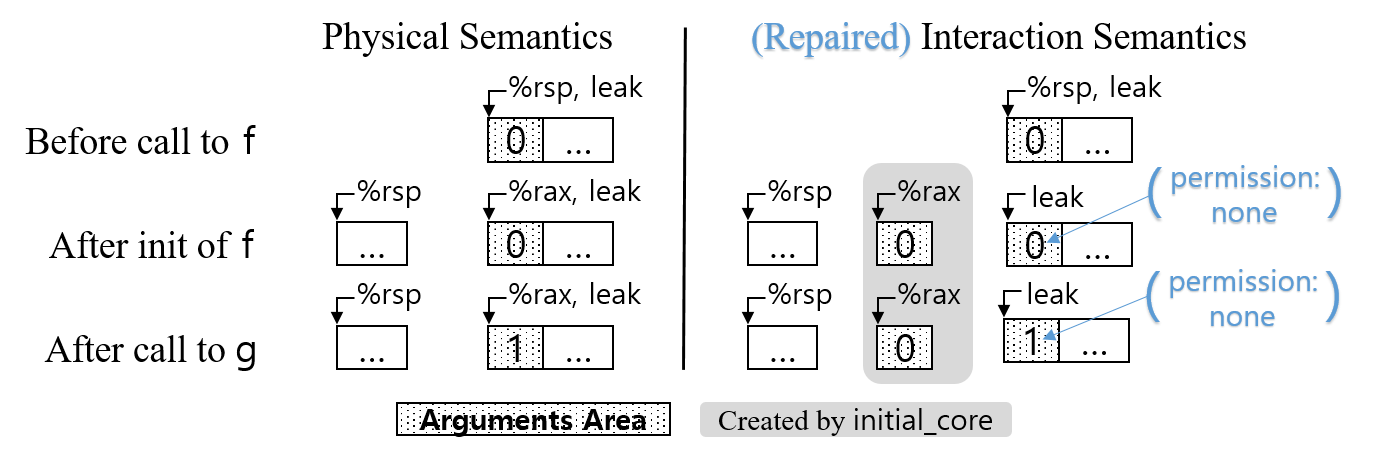
\includegraphics[width=.983\textwidth]{images/ex-stack.png}}
\end{minipage}
%% \fbox{\begin{minipage}{.8pc}\mbox{}\\[4.53mm](c)\\[3.73mm]\mbox{}\end{minipage}}
%% \hspace*{-1.9mm}
%% \begin{minipage}{.95\textwidth}
%%   \begin{Verbatim}[frame=single]
%%                      Physical Semantics         Interaction Semantics
%%                             %rsp           |                  %rsp       
%% Before call to f:           [=0=| ... ]    |                  [=0=| ... ]
%%                     %rsp    %rax           |    %rsp    %rax             
%%  After init of f:   [ ... ] [=0=| ... ]    |    [ ... ] [=0=] [=0=| ... ]
%%                     %rsp    %rax           |    %rsp    %rax             
%%  After call to g:   [ ... ] [=1=| ... ]    |    [ ... ] [=0=] [=1=| ... ]
%%   \end{Verbatim}
%% \end{minipage}
\caption{A counterexample showing the problem with the assumption on the stack}
\label{fig:stack-convention}
\end{figure}

\myparagraph{Counterexamples}
%
The example in \Cref{fig:stack-convention} shows how violations of the assumption
can invalidate correct compiler translations.
%
The box~(a) shows handwritten assembly code implementing two functions
\texttt{main} and \texttt{g}; the box~(b) shows a standard translation
of C code into assembly essentially performed by \texttt{gcc -O0}; and
the left-hand side (LHS) of the box~(c) depicts the shape of the stack
during execution in the physical semantics.
The function \texttt{main} stores the address of the
outgoing arguments area (\ie \texttt{\%rsp} as depicted in LHS of (c))
in the global variable \texttt{leak} and invokes the function
\texttt{f}, where the last argument \texttt{0} is stored in the
arguments area of the stack. Then the function \texttt{f} makes three
function calls, \texttt{out(x)}, \texttt{g()} and \texttt{out(x)},
where the argument \texttt{x} is directly read from the arguments area
pointed to by \texttt{\%rax} in the assembly, as depicted in LHS of
(c), and \texttt{out(x)} outputs the read value.  Finally, the
function \texttt{g} updates the arguments area pointed to by
\texttt{leak} with~\texttt{1}, as depicted in LHS of (c), between the
two function calls \texttt{out(x)}.

An important point here is that the compiler assumes that the
arguments area (\ie \texttt{\%rax}) is unchanged across the
function call \texttt{g()} since it is fully owned by \texttt{f}.
Therefore, the compiler expects that both calls
\texttt{out(*(\%rax))} in the target code correctly output
\texttt{0}. However, since the function \texttt{g} updates the
arguments area with \texttt{1} via \texttt{leak}, the two calls
incorrectly output \texttt{0} and~\texttt{1}.
We confirmed this incorrectness by
compiling \texttt{f} with \texttt{gcc -O2}, which
eliminates the second load \texttt{*(\%rax)} by propagating
the result of the first load across \texttt{g()}
thereby outputting \texttt{0} twice.

\myparagraph{Our Model}
%
In order to solve the problem, we have to distinguish accesses to the
arguments area via the caller from those via the callee and define the
former as UB. Though making such distinction is difficult in the
physical semantics, fortunately it is already made in interaction
semantics due to the language-independent design. For example, consider
the interaction semantics of the above example, depicted in the
right-hand-side (RHS) of \Cref{fig:stack-convention}~(c).  The
difference is that when the assembly function \texttt{f} is invoked,
the initialization process (\ie \texttt{init\_core}) of the module
semantics newly constructs the arguments area of the stack from the
given logical arguments in order to make an environment needed to
execute the assembly function \texttt{f}. This is essentially needed
because the caller may not be an assembly module so that it may not
have its own stack at all.  Then the callee sees the new arguments
area created by \texttt{init\_core} while the caller (in assembly)
sees the original arguments area.

Although the original interaction semantics does not prevent access to
the arguments area via the caller, we can easily fix it.
%% Now we can easily repair the original interaction semantics to make
%% those accesses to the arguments area via the caller as UB during the
%% lifetime of the callee.
We simply $(i)$ turn off the access
permission of the original arguments area in the \texttt{at\_external}
step of the caller module, and $(ii)$ turn it back on in the
\texttt{after\_external} step. Note that the notion of permission
%% is already an existing feature of
already exists in the \cc{} semantics, so that we do not
need to strengthen it. In the above example again,
the update by \texttt{g} will raise UB since the original argument area pointed
to by \texttt{leak} has no access permission.

%% \jeehoon{I think the idea of repairing interaction semantics is a little bit abrupt.  I think it's
%%   necessary to explain why interaction semantics is wrong.}

\hide{

\todo{Interaction Semantics and UB}

\myparagraph{Correctness Statement}
%
\ccc{}'s correctness also establishes behavioral refinement. To be
specific, consider a source program consisting of C modules
$\texttt{s}_1\texttt{.c},\ldots,\texttt{s}_n\texttt{.c}$ and assembly
modules $\texttt{a}_1\texttt{.asm},\ldots,\texttt{a}_m\texttt{.asm}$.
Now suppose
$\texttt{t}_1\texttt{.asm},\ldots,\texttt{t}_n\texttt{.asm}$ are the
assembly modules separately compiled from the source C modules by the
\cc{} compiler. The correctness of this compilation says that the
observable behaviors of the target assembly consisting of
$\texttt{t}_1\texttt{.asm},\ldots,\texttt{t}_n\texttt{.asm}$,
$\texttt{a}_1\texttt{.asm},\ldots,\texttt{a}_m\texttt{.asm}$ is
included in that of the source program according to \emph{interaction
  semantics} described below.

\begin{figure}[t]%% {0.43\textwidth}
  \centering
  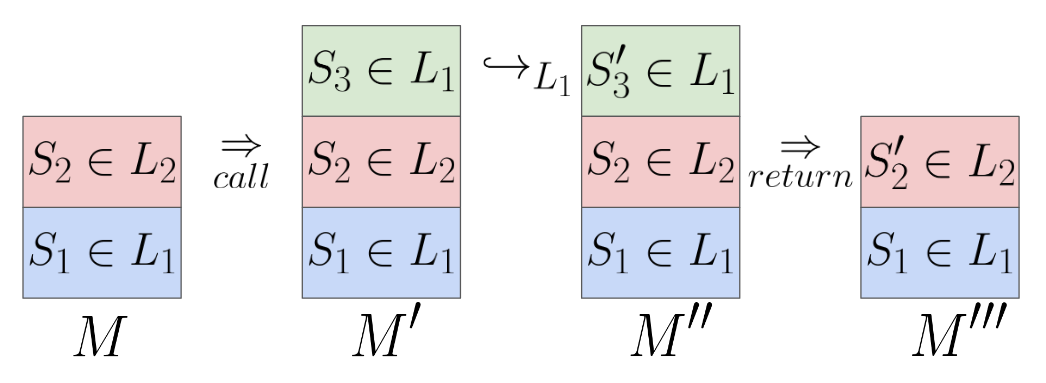
\includegraphics[width=0.7\linewidth]{images/interaction-semantics2.png}
  \caption{}
\label{fig:interactionsemantics}
\end{figure}

Interaction semantics gives a mathematical model for executing
multi-language programs by providing a general mechanism that defines
intermodule steps, while defining intramodule steps according to the
underlying language's semantics.
\todo{
  revise the following: main points
  - copying module states for generality
  - C, assembly, ILs share the same notion of memory
  - marshalling, unmarshalling and making environment for the module (the underlying language assumes the uni-language setting.) --> change memory at intermodule steps
}
%
\Cref{fig:interactionsemantics} illustrates how interaction semantics works.
%% As illustrated in \Cref{fig:interactionsemantics},
The state of interaction semantics consists of a \emph{shared} memory, and a stack of language-local states \emph{without} memory.
The notion of shared memory is legitimate because every language of \cc{} shares the same notion of memory.
%% Note that every language of \cc{} shares the notion of memory, and hereafter we use $\States{\mathbb{L}}$ to denote a language-local state \emph{without} memory (\eg local variable mapping for C and register set for assembly).
Intermodule steps pushes or pops the stack (at call case and return case, respectively) while intramodule steps just changes the topmost state of the stack.
%% Intermodule steps are divided into two kinds, namely call and return, each pushing and popping the stack.
%% Intramodule steps does not push or pop the stack, instead it just updates the topmost state of the stack.
%% \Cref{fig:interactionsemantics} illustrates these in more detail.

\youngju{multi-language program? multi-module program?}

%% During its execution, $S_2$ encounters a call to an external function.
Note that, in order to define intermodule steps modularly, a representation of function arguments is globally fixed ($\overrightarrow{val}$).
Therefore, when $S_2$ encounters a call to an external function, $L_2$ \emph{marshall}s arguments from its language-local representation to global representation before passing them.
Then $L_3$ receives the arguments and \emph{unmarshall}s those to its language-local representation and initializes a new state with it, resulting in $S_3$.
An intramodule step of $S_3$ proceeds by just reusing its language-local step, $\estep{}_3$.
When $S_3'$ returns, similarly with call case, the return value is passed to $S_2$ (through marshalling and unmarshalling) and its state is updated correspondingly.


%% ($S_i \in \States{\mathbb{L}_i}$)

%% The left arrow and right arrow each depicts intermodule step,
%% When a function from another module is called during its execution,
%% During its execution, a function from another module is called during execution, a new
%% $S_2$
%% When an external module is called,
%% There are two kinds of intermodule steps, namely call and return, each pushing and popping
%% \youngju{처음부터 memory 분리?}
%% the intermodule step is divided into \emph{call} and \emph{return}, each pushing or popping
%% As illustrated in \Cref{fig:interactionsemantics}, the intermodule step is divided into \emph{call} and \emph{return}, each pushing or popping

\todo{Discuss advantages of interaction semantics, here or intro?}

\subsection{Semantic Techniques}\label{sec:background:ub}

Common compiler optimizations are not always correct in general for
all well-typed C programs because the syntactic type checking cannot
rule out all semantically invalid programs. In order to rule out such
invalid programs thereby making those optimizations correct, \cc{}
uses two semantic techniques, \emph{undefined behavior} and
\emph{logical memory}. In addition, to model uninitialized values,
\cc{} uses the notion of \emph{undefined value}.

\myparagraph{Undefined Behavior}
%
The main idea for ruling out invalid programs is to raise
\emph{undefined behavior (UB)} during execution if an undesirable
operation occurs, where UB is interpreted as producing all possible
traces of events.  Then for correctness of optimizations, it suffices
to prove behavioral refinement until UB happens because, once it
happens, behavioral refinement holds trivially.
As an example, consider the following program.
%
\[
\begin{minipage}{0.4\textwidth}
\begin{verbatim}
int arr[1], x = 0;
*(arr+1) = 1;
out(x); // optimizes to "out(0)"
\end{verbatim}
\end{minipage}
\]
%
Here \cc{} optimizes \texttt{out(x)} to \texttt{out(0)} by
propagating the initial value of \texttt{x} because a simple analysis
indicates that the variable \texttt{x} is not modified.  However, this
analysis would be invalidated in a naive semantics.  For example,
suppose \texttt{arr} and \texttt{x} are allocated at \texttt{0x100}
and \texttt{0x104}. Then the out-of-bound access \texttt{*(arr+1) = 1}
updates \texttt{x} with \texttt{1} thereby making the optimization
incorrect.  \cc{} solves this problem by defining such out-of-bound
access as undefined behavior.

Now the question is how to define out-of-bound access. To see the
problem, consider the two accesses \texttt{*(arr+1)} and \texttt{*(\&x)}
in the above example. Though \texttt{arr+1} and \texttt{\&x} are exactly
the same address \texttt{0x104}, one should be able to distinguish them:
the former access as out-of-bound but the latter not.

%% As an example,
%% consider a simple optimization translating \texttt{x+1 > x} to
%% \texttt{true}. \todo{revise:}
%% Note that if \code{x} was \code{INT\_MAX}, the inequality does not hold because of an integer overflow.
%% Therefore, such invalid operation (triggering overflow) is defined as UB so that the optimization is justified.

\myparagraph{Logical Memory}
%
To address this problem, \cc{} introduces the notion of \emph{logical
  memory}, which models the memory as a set of independent blocks and
pointer values as pairs of a block identifier and an offset inside the
block. In the previous example, two logical blocks of size 1 are
allocated: one for \texttt{arr} with identifier, say \texttt{bid 10},
and the other for \texttt{x} with identifier, say \texttt{bid
  11}. Then the addresses \texttt{arr+1} and \texttt{\&x} are
distinguished as \texttt{(bid 10,1)} and \texttt{(bid 11,0)}, where
the former is clearly out-of-bound but the latter not because the
blocks are of size 1.

%% \youngju{전달할 이야기: (i) private protection이 중요 (ii) 메모리 기본 연산들 (alloc, free) 이 동작하는 방식? (marshall/unmarshall)}

%% \youngju{invalid access 라고 뭉뚱그려 말한 이유: dangling pointer 등도 UB를 잘 준다.}

%% \youngju{free 설명할 때 dangling pointer로 설명?}

%% \youngju{https://hal.inria.fr/hal-00703441/document 보고 써서 문장이 비슷한데 paraphrase 더 해야 할 수도}

%% \youngju{여기만 생각하면 separation만 가지고 설명해도 충분한데, 위에서 out-of-bound access 이야기랑 맞춰야 함}

%% \youngju{primitive operation 이야기: 우리는 하나 늘린 셈 (unfree). 이게 장점인지 단점인지}

%% \youngju{alloc이 사실은 Z 두개 받는데, \Cref{fig:logical-memory}랑 안헷갈리게 하나로 함}

\myparagraph{Undefined Value}
%
\todo{
  - uninitialized value -> undefined value
  - undefined value -> propagate; observe on UV -> UB
  - As a result, one can optimize UV to any value.
  - Note that modeling uninitialized value as assigning arbitrary values nondeterministically
    or branching on UV as branching either way nondeterministically
    is not an option for \cc{} because the language should deterministic in order to use forward simulation as discussed in Section blah.
}


} %\hide 

\hide{

\subsection{Applications}

%% The root cause of such overhead is that their verification technique
%% was not flexible: a single memory relation is enforced for every
%% per-pass correctness proof. In contrast, \cc{} employs three different
%% memory relations so that each pass can be proven with the simplest but
%% sufficient one. In other words, their approach failed to achieve
%% \emph{true vertical compositionality}\cite{TODO}.

%% To address this problem, we developed new proof techniques that allow
%% lightweight verification with focus on minimizing language-specific
%% and pass-specific developments. First one is end-language contextual
%% refinement, which recovers the flexibility to chose a convenient
%% memory relation. Second one is mixed simulation, which tames the
%% nondeterminism introduced in \Cref{sec:overview-semantics}. The last
%% one is an analysis framework to address a new challenge about modular
%% verification of modular analysis. \todo{why new? introduced recently}

To address this problem, we developed new proof techniques that allow
lightweight verification with focus on minimizing language-specific
and pass-specific developments. First one is end-language contextual
refinement, which addresses the root cause of \ccc{}'s overhead:
vertical composition (of simulation relation).
%% it
%% fixed \emph{single}, sophisticated memory relation for every per-pass
%% proof, while \cc{} employs three different ones so that each per-pass
%% proof uses sufficient but simplest one.
Second one is mixed simulation, which tames the nondeterminism we
introduced in \Cref{sec:overview-semantics}. The last one is a local
preservation, which supports verification of modular analysis which
was introduced in \cc{} since \ccc{} was no longer maintained.

As a result, we successfully reused \cc{}'s developments and our
development comprises 48K lines of Coq (25.4\% compared to the
baseline) where language-specific or pass-specific developments are
only 11K lines of Coq (13.3\% compared to corresponding baseline).
%order-of-magnitue smaller?

\vspace{5mm}
\begin{tabular}{ c || c | c || c | c }
  portion
  &
  \ccc{}
  &
  \cc{} 2.1
  &
  \ccm{}
  &
  \cc{} 3.5
  \\
  \hline
  language/pass-specific
  &
  +76,973 (125.8\%)
  &
  61,196
  &
  +11,339 (13.3\%)
  &
  85,056
  %% \\
  %% others (TODO: remove?)
  %% &
  %% +45,304
  %% &
  %% 50,925
  %% &
  %% +36,956
  %% &
  %% 105,048
  \\
  whole
  &
  +122,277 (109.1\%)
  &
  112,125
  &
  +48,295 (25.4\%)
  &
  190,104
\end{tabular}
\vspace{5mm}

As a consequence, the intermodule case of the local simulation can be
established \emph{assuming} the source state is sound (just as in
whole-program simulation), as the preservation of sound-state is
provided by local-preservation. Of course, the horizontal composition
of local simulations now additionally require local preservations of
each end language, which will actually be just C, RTL (a target
language of analyzers), and assembly thanks to ELCR.

\note{without ./bounds/, 41424}

\note{counted only x86 directory. should we mention it?}

\note{v3.5 has parser.v (34083 LOC) and v2.1 does not.}

\todo{1,000 or 1000?}

\todo{show the number without Stackingproof.v?}



\todo{위: re-implementation of each language’s semantics and each passes’ proof
  아래: language-specific or pass-specific developments}

%쓰이는 표현임: Not by Power, Nor by Might, but by My Spirit
%lines of Coq: sepcomp에서 쓰임
%evolve over time 쓰임
%In response: viktor abstract에서 씀
%10331.0 / 79488

\todo{
Except for the initial state, every other state remains deterministic,
and we were able to reuse existing proof at ease.  As a consequence,
we successfully reused existing proof.
}








%% 우리가 추가한 nondeterminisim은 오직 assembly가 시작할 때 뿐이고, 나머지 부분은 여전히 deterministic하다.
%% 이 local determinisim을 이용해서 2-b)로 논증하면, 기존 forward simulation을 성공적으로 재사용할 수 있다.




\subsection{Defining a Sound and General Semantics}\label{sec:overview:semantics}
In this subsection, we describe challenges on defining a sound and general multi-language semantics for C and assembly, and show our solution.
By \textit{sound}, we mean its behavior contains actual behavior when ran on the machine.
By \textit{general}, we mean it should support arbitrary program.
%% that is \textit{general}, \eg{} supporting \textit{arbitrary}
We elide some technical subtleties for the sake of simplicity.
In \Cref{TODO}, we provide technically more complete argument for a curious reader.

\subsection{Register (tentative)}\label{sec:overview:register}
\myparagraph{Problem (tentative)}
%% %% \chapter{\;\;\;\;Compiler Verification: CompCertM} %%이러면 (toc 말고 본문에서) 넘침
\chapter{\;\;\;\;Compiler Verification}
\label{sec:compiler}

\section{Background}
\label{sec:compiler:background}

\subsection{A Brief Introduction on CompCert}

\myparagraph{Undefined Behavior}



\section{Problems}
\label{sec:compiler:problems}

The problems with the interaction semantics of \ccc{} are that it does
not satisfy two adequacy properties. First, the adequacy w.r.t. C says
that for any C modules $M_1,\ldots,M_n$, the behaviors of the linked
program according to interaction semantics $\beh{M_1 \llink
  \ldots \llink M_n}$ should \emph{be included in} those according to the
physical semantics $\beh{M_1 \plink \ldots\plink M_n}$.  The reason for
failure was quite simple and we could easily fix it: unlike \ccc{}, we allow passing
the \texttt{undef} value to an external module since the C semantics
does so, while we turn ill-typed values into \texttt{undef} when they
are passed to an external module.

Second, the failure of the adequacy w.r.t. assembly is more serious.
Adequacy says that for any assembly modules $M_1,\ldots,M_n$,
the behaviors of the linked program according to interaction
semantics $\beh{M_1 \llink \ldots \llink M_n}$ should \emph{include}
those according to the physical semantics $\beh{M_1 \plink \ldots\plink M_n}$.
Note that the direction is opposite since assembly is the target language.
As discussed before, the reason for failure is that
the interaction semantics of \ccc{} does not have a mechanism to detect
illegal interference and make it undefined behavior~(UB).

\section{Solution}
\label{sec:compiler:solution}

We identify the sources of inadequacy w.r.t. assembly as violations of
three assumptions made by standard compilers: two on the registers and one on the stack.
We discuss why they 
cause problems with counterexamples and show how to semantically
handle them without changing the underlying language semantics.

\subsection{Assumptions on the Registers}
\label{sec:overview-semantics-register}
%
The two problematic assumptions on the registers are that
an invoked assembly function $(i)$ should
preserve the initial values of the callee-save registers, and $(ii)$
should not access the memory via the leftover pointer values remaining
in those registers that are not involved in passing meaningful information to the callee,
which we henceforth call \emph{\nip{}} registers.
%% in those registers, which we call \emph{non-passing} registers,
%% that are not involved in passing information to the callee.
%% the \emph{non-passing} registers (\ie those registers not involved
%% in passing information to the callee).
%% We discuss these two conventions together because it is nontrivial to find a
%% single model that enforces both conventions at the same time.
%% \jeehoon{I don't understand the last sentence..}
%% \jeehoon{``\nip{}'': how about ``opaque''?}

\begin{figure}[t]
\fbox{\begin{minipage}{.9pc}\mbox{}\\[15.25mm](a)\\[13.45mm]\mbox{}\end{minipage}}
\hspace*{-2.7mm}
\begin{minipage}{0.70\textwidth}
\begin{Verbatim}[frame=single]
int main()   {          main:
  int* x = malloc(8);     ...
  x[0] = 0;               *(%rbx) = 0;
  x[1] = 1;               *(%rbx + 4) = 1;
  f();               -->  f();
  out(x[0]);              out(*(%rbx));
  ...                     ...
}
\end{Verbatim}
\end{minipage}
$\mbox{}~\mathlarger{\mathlarger{\mathlarger{\mathlarger{\mathlarger{\llink}}}}}~\mbox{}$
\\
\vspace{3mm}
\\
\fbox{\begin{minipage}{.9pc}\mbox{}\\[10.50mm](b)\\[8.70mm]\mbox{}\end{minipage}}
\hspace*{-2.7mm}
\begin{minipage}{0.33\textwidth}
\begin{Verbatim}[frame=single]
f:
  if (g(%rbx))
    %rbx = %rbx + 4;
  else
    *(%rbx) = 1;

\end{Verbatim}
\end{minipage}
\caption{A counterexample showing the problem with the assumptions on the registers}
\label{fig:reg-convention}
\end{figure}

\myparagraph{Counterexamples}
%
The example in \Cref{fig:reg-convention} shows how violations of the two
assumptions can invalidate correct compiler translations.
%% \jeehoon{I think counterexample should go to the problems section.}
%
The code in the left box~(a) shows a standard translation of C code into assembly
(written in pseudocode) performed by mainstream compilers like GCC and LLVM, where the accesses to
the array \texttt{x} are translated into accesses via the register
\texttt{\%rbx} assuming that \texttt{\%rbx} is set to contain the
address of \texttt{x}. An important point here is that the compiler
assumes that $(i)$ the value of \texttt{\%rbx} is unchanged across
the function call \texttt{f()} since it is a callee-save register,
and also $(ii)$ the values in the array pointed to by \texttt{\%rbx} are
unchanged across \texttt{f()} since the array's addresses do not escape
except via \nip{} registers like \texttt{\%rbx}.
Therefore, the compiler expects that \texttt{out(*(\%rbx))} in the target code
correctly outputs \texttt{0}.

The right box~(b) presents an example of handwritten assembly
(written in pseudocode) for function \texttt{f} that violates the
above two assumptions of the compiler. The code either increments
\texttt{\%rbx} by \texttt{4} or writes \texttt{1} to \texttt{*(\%rbx)}
depending on the result of call to \texttt{g}.  Now if we link the assembly
code in (a) and that in (b) together, one can easily see that
\texttt{out(*(\%rbx))} incorrectly outputs~\texttt{1} instead
of \texttt{0} in either case: in the former case, \texttt{\%rbx}
points to the second element of the array~\texttt{x}, which contains
\texttt{1}; in the latter case, the value of \texttt{*(\%rbx)} is
directly updated to \texttt{1}. Therefore, it makes sense to
define those illegal behaviors of (b) as undefined behavior~(UB).

\myparagraph{Our Model}
\label{sec:compiler:solution:model}
%
We present our model making the illegal behaviors UBs
in stages, explaining at each stage why naive models do not work.
%% \jeehoon{What's the difference between ``stage'' and ``state''?}
%% \jeehoon{We have ``Our Solution'' paragraph inside ``Our Solution'' section. How about moving
%%   counterexample to the problems section, and giving a paragraph to each stage?}

First, in order to enforce the preservation of callee-save register
values, we store the initial values of the callee-save registers at
the \texttt{init-core} step of assembly modules; and check, at the
\texttt{halted} step, whether the final values of those registers are
equal to the stored initial values and if not, raise UB.  Here, the
question is, when a new core with a fresh register file is pushed into the core stack,
what values should be set as initial values of the \nip{}
registers including all of the callee-save registers.  Since the
registers may contain arbitrary values in the physical assembly
semantics, a natural choice would be to initially set them to contain
the \texttt{undef} value, which is an abstract value representing all
possible values. Indeed, this is the choice of \ccc{}.  However, there
is a serious problem. Since, for instance, \texttt{undef + 4} results
in \texttt{undef}, checking whether the final values of callee-save
registers are equal to the initial values, \ie \texttt{undef}, is
not sufficient. Specifically, the assembly code in (b) above
does not raise UB in this new semantics in case \texttt{g(\%rbx)} returns \texttt{1}
because the initial and final values of \texttt{\%rbx}
are both \texttt{undef} and thus equal
even though the callee-save register \texttt{\%rbx} is incremented
by \texttt{4} in the physical semantics.

Second, another natural solution would be to initially set the
\nip{} registers to nondeterministically contain arbitrary
values including \texttt{undef}. Though this model is more flexible,
it still has a problem. For instance, in the above example, to
simulate the physical behaviors of the assembly function \texttt{f} in
interaction semantics, one can set the initial value of \texttt{\%rbx} to
be either $(i)$ \texttt{undef} (\ie a more abstract value than the physical one), or
$(ii)$ a pointer to the array \texttt{x} (\ie a value equivalent to the physical one):
other values cannot be used since they are not refined by the value of \texttt{\%rbx} in the target,
which is required since the value is passed to an unknown function~\texttt{g}.
In the former case, if
\texttt{g(\%rbx)} returns \texttt{1}, we have the same problem with
callee-save checking as shown above.  In the latter case, if
\texttt{g(\%rbx)} returns \texttt{0}, the function \texttt{f}
successfully updates the array~\texttt{x} thereby invaliding the
translation in (a) as illustrated above.

We solve this problem by further revising the second model:
nondeterministically allocating an arbitrary number of \emph{junk
  blocks} (\ie blocks of size zero) and then initializing the
\nip{} registers with arbitrary non-pointer values or
\emph{junk pointers} (\ie pointers to the junk blocks).  Then we can
simulate the physical behaviors by initializing each register $r$
$(i)$ with the same non-pointer value if the physical value of $r$ is
a non-pointer value; and $(ii)$ otherwise with a fresh junk pointer.
The high-level idea is that, like \texttt{undef}, a junk pointer is
more abstract (\ie causing more UBs) than any pointer but, unlike
\texttt{undef}, sufficiently distinguishable. For instance,
in the previous example, if \texttt{g(\%rbx)} returns \texttt{1},
the initial and final values of \texttt{\%rbx} (\ie $p$ and $p+4$ for a junk pointer $p$)
are distinguished thereby raising UB by the callee-save checking;
if \texttt{g(\%rbx)} returns \texttt{0},
the memory access \texttt{*(\%rbx) = 1} raises UB because \texttt{\%rbx}
points to a junk block of size zero.

Finally, note that introducing nondeterminism as above is not a
showstopper thanks to the mixed simulation, as discussed in
\Cref{sec:overview-verification:mixedsim}: we can do forward
simulation everywhere except for the \texttt{init\_core} step of
assembly modules, where we should do backward simulation.

\subsection{Assumptions on the Stack}
\label{sec:overview-semantics-memory}
%
The problematic assumption on the stack is that the
\emph{outgoing arguments area} of a caller's stack (\ie where overflowing function
arguments are stored) should be fully \emph{owned} by the callee. In
other words, the callee can assume that the arguments area is never
modified by others unless its addresses are revealed to the public by
the callee itself.

\begin{figure}[t]
\fbox{\begin{minipage}{.9pc}\mbox{}\\[10.45mm](a)\\[8.65mm]\mbox{}\end{minipage}}
\hspace*{-1.9mm}
\begin{minipage}{0.255\textwidth}
  \begin{Verbatim}[frame=single]
main:
  ...  
  leak = %rsp;
  f(..., 0);
g:
  *leak = 1;
  \end{Verbatim}
\end{minipage}
$\mbox{}~\mathlarger{\mathlarger{\mathlarger{\mathlarger{\mathlarger{\llink}}}}}~\mbox{}$
\fbox{\begin{minipage}{.9pc}\mbox{}\\[10.45mm](b)\\[8.65mm]\mbox{}\end{minipage}}
\hspace*{-1.9mm}
\begin{minipage}{0.695\textwidth}
  \begin{Verbatim}[frame=single]
void f(..., int64_t x)       f:
{                              ...
  out(x);                      out(*(%rax));
  g();                  -->    g();
  out(x);                      out(*(%rax));
}                              ...
  \end{Verbatim}
\end{minipage}
\\[1mm]
\fbox{\begin{minipage}{.9pc}\mbox{}\\[15.90mm](c)\\[15.10mm]\mbox{}\end{minipage}}
\hspace*{-2.7mm}
\begin{minipage}{.95\textwidth}
\fbox{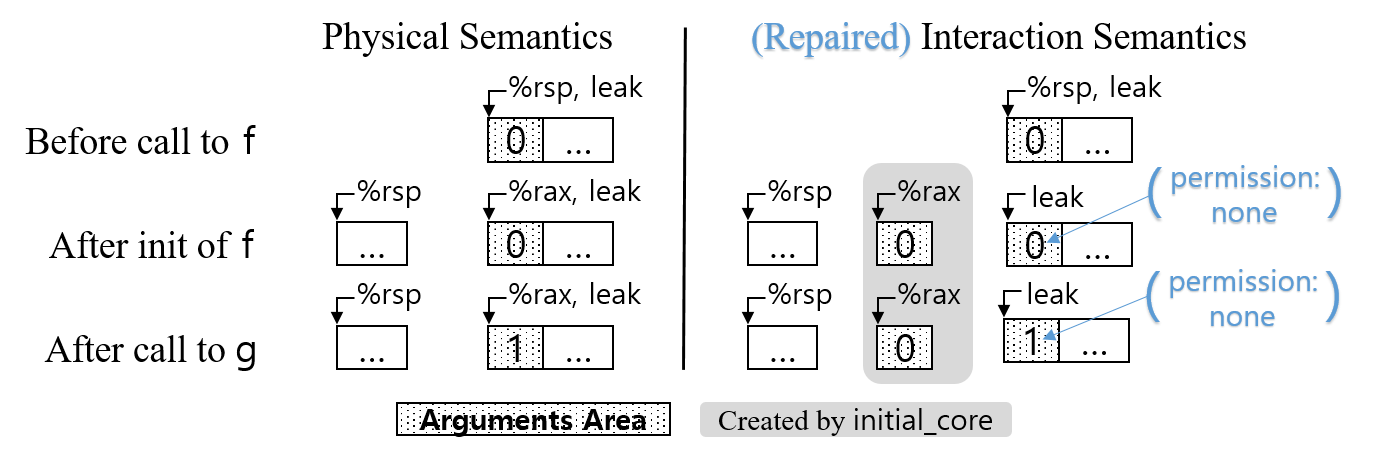
\includegraphics[width=.983\textwidth]{images/ex-stack.png}}
\end{minipage}
%% \fbox{\begin{minipage}{.8pc}\mbox{}\\[4.53mm](c)\\[3.73mm]\mbox{}\end{minipage}}
%% \hspace*{-1.9mm}
%% \begin{minipage}{.95\textwidth}
%%   \begin{Verbatim}[frame=single]
%%                      Physical Semantics         Interaction Semantics
%%                             %rsp           |                  %rsp       
%% Before call to f:           [=0=| ... ]    |                  [=0=| ... ]
%%                     %rsp    %rax           |    %rsp    %rax             
%%  After init of f:   [ ... ] [=0=| ... ]    |    [ ... ] [=0=] [=0=| ... ]
%%                     %rsp    %rax           |    %rsp    %rax             
%%  After call to g:   [ ... ] [=1=| ... ]    |    [ ... ] [=0=] [=1=| ... ]
%%   \end{Verbatim}
%% \end{minipage}
\caption{A counterexample showing the problem with the assumption on the stack}
\label{fig:stack-convention}
\end{figure}

\myparagraph{Counterexamples}
%
The example in \Cref{fig:stack-convention} shows how violations of the assumption
can invalidate correct compiler translations.
%
The box~(a) shows handwritten assembly code implementing two functions
\texttt{main} and \texttt{g}; the box~(b) shows a standard translation
of C code into assembly essentially performed by \texttt{gcc -O0}; and
the left-hand side (LHS) of the box~(c) depicts the shape of the stack
during execution in the physical semantics.
The function \texttt{main} stores the address of the
outgoing arguments area (\ie \texttt{\%rsp} as depicted in LHS of (c))
in the global variable \texttt{leak} and invokes the function
\texttt{f}, where the last argument \texttt{0} is stored in the
arguments area of the stack. Then the function \texttt{f} makes three
function calls, \texttt{out(x)}, \texttt{g()} and \texttt{out(x)},
where the argument \texttt{x} is directly read from the arguments area
pointed to by \texttt{\%rax} in the assembly, as depicted in LHS of
(c), and \texttt{out(x)} outputs the read value.  Finally, the
function \texttt{g} updates the arguments area pointed to by
\texttt{leak} with~\texttt{1}, as depicted in LHS of (c), between the
two function calls \texttt{out(x)}.

An important point here is that the compiler assumes that the
arguments area (\ie \texttt{\%rax}) is unchanged across the
function call \texttt{g()} since it is fully owned by \texttt{f}.
Therefore, the compiler expects that both calls
\texttt{out(*(\%rax))} in the target code correctly output
\texttt{0}. However, since the function \texttt{g} updates the
arguments area with \texttt{1} via \texttt{leak}, the two calls
incorrectly output \texttt{0} and~\texttt{1}.
We confirmed this incorrectness by
compiling \texttt{f} with \texttt{gcc -O2}, which
eliminates the second load \texttt{*(\%rax)} by propagating
the result of the first load across \texttt{g()}
thereby outputting \texttt{0} twice.

\myparagraph{Our Model}
%
In order to solve the problem, we have to distinguish accesses to the
arguments area via the caller from those via the callee and define the
former as UB. Though making such distinction is difficult in the
physical semantics, fortunately it is already made in interaction
semantics due to the language-independent design. For example, consider
the interaction semantics of the above example, depicted in the
right-hand-side (RHS) of \Cref{fig:stack-convention}~(c).  The
difference is that when the assembly function \texttt{f} is invoked,
the initialization process (\ie \texttt{init\_core}) of the module
semantics newly constructs the arguments area of the stack from the
given logical arguments in order to make an environment needed to
execute the assembly function \texttt{f}. This is essentially needed
because the caller may not be an assembly module so that it may not
have its own stack at all.  Then the callee sees the new arguments
area created by \texttt{init\_core} while the caller (in assembly)
sees the original arguments area.

Although the original interaction semantics does not prevent access to
the arguments area via the caller, we can easily fix it.
%% Now we can easily repair the original interaction semantics to make
%% those accesses to the arguments area via the caller as UB during the
%% lifetime of the callee.
We simply $(i)$ turn off the access
permission of the original arguments area in the \texttt{at\_external}
step of the caller module, and $(ii)$ turn it back on in the
\texttt{after\_external} step. Note that the notion of permission
%% is already an existing feature of
already exists in the \cc{} semantics, so that we do not
need to strengthen it. In the above example again,
the update by \texttt{g} will raise UB since the original argument area pointed
to by \texttt{leak} has no access permission.


\subsection{Mixed Simulation}
\label{sec:overview-verification:mixedsim}

While the target language of \cc{} is deterministic (more precisely,
the source is receptive and the target is determinate) thereby mostly
using forward simulations, the repaired interaction semantics of
\ccm{} is inherently nondeterministic to handle illegal interference from assembly modules
%% enforce the assembly calling conventions
(\Cref{sec:compiler:solution:model}) thus preventing the
use of forward simulation.
%% While it is theoretically possible to convert the \cc{}
%% verification from forward to backward simulations, it would incur a
%% significant cost since a compiler pass typically compiles a single
%% instruction in the source down to several instructions in the target.
%% %% due to the nature of source and target languages and the size of verification.
%% For this reason, determinism
%% has been considered ``instrumental for the simulation proofs of the compiler passes and its absence
%% is a show stopper''~\cite{besson:intptr}.
% Extending \cc{}'s semantics with such nondeterministic features can potentially cause significant
% overhead, as it invalidates forward simulation and enforces one to use backward simulation, which
% effectively means one should re-establish simulation proof from the scratch.  In literature, it is
% even said that

In order to recover the ability to use forward simulation in the occasional presence of nondeterminism,
we adopt the idea of \emph{mixed (forward-backward) simulation} from \cite{neis:pilsner}.
%% To embrace nondeterminism with low verification cost, we develop more general simulations, called
%% \emph{mixed simulations}, that (mostly) allow forward reasoning in the (occasional) presence of
%% nondeterminism.
The key observation is that
the requirement for using forward simulations (\ie determinism of the target) is a per-state property,
not a per-language property: as long as a particular target machine state is \emph{locally deterministic} (\ie its next state is unique),
one can do forward simulation at that state.
%% conversion from backward to forward simulations
%% requires only the current target \emph{machine state}, not the entire target \emph{language}, to be
%% deterministic.
Based on this observation, mixed simulations selectively allow forward
simulation when the target is locally deterministic, in addition to
the default backward simulation.
%% for each pair of related machine states, we allow the verifier to
%% \emph{choose} to perform either forward or backward reasoning, requiring that forward reasoning is
%% used only for locally deterministic target machine states.
%
Specifically, we say that a relation $R$ is a (closed) mixed simulation if
for all $(\mssrc, \mstgt) \in R$,
%% \makebox[\linewidth]{\makebox[1.2\linewidth]{
%% \begin{minipage}{1.2\linewidth}
\begin{enumerate}
\item
  $\forall e, \mstgt',~ \mstgt \estep{e} \mstgt' \implies {} $ \\
  $ \exists \mssrc',~ \mssrc \estep{\tau}^{\raisebox{-1mm}{\scriptsize$\ast$}} \estep{e}\estep{\tau}^{\raisebox{-1mm}{\scriptsize$\ast$}} \mssrc' \land (\mssrc', \mstgt') \in R$; or
\item
  $\forall e, \mssrc',~ \mssrc \estep{e} \mssrc' \implies {} $ \\
  $ \exists \mstgt',~ \mstgt \eustep{\tau}^{\raisebox{-1mm}{\scriptsize$\ast$}} \eustep{e}\eustep{\tau}^{\raisebox{-1mm}{\scriptsize$\ast$}} \mstgt' \land (\mssrc', \mstgt') \in R$\\
\end{enumerate}
%% \end{minipage}
%% }}
where $\ms \eustep{e} \ms'$ denotes that $\ms$ is locally deterministic and $\ms \estep{e} \ms'$.

\Cref{fig:mixedsim} visualizes this formulation of mixed simulation, where
%% presents an example of mixed simulations, where $R$ is a simulation relation; red and blue circle represent source and
%% target machine states, respectively;
solid and dotted arrows represent universally and existentially
quantified steps, respectively, and double circles represent locally
deterministic target states. In this figure,
since the first three target machine states are deterministic,
we can do forward simulation as shown in the figure;
then, since the following target state is nondeterministic,
we should do backward simulation as shown in the figure.
%% the first three target machine states are deterministic.  The
%% first three target steps are deterministic and reasoned in a forward manner (from source to target),
%% and the last target step is nondeterministic and reasoned in a backward manner (from target to
%% source).  Later, those part of simulations that are reasoned in a forward manner is converted to
%% backward reasoning, thereby proving backward simulation and thus behavior refinement.

Note that the repaired interaction semantics is nondeterministic only
at the initial step of a module invocation, so that we can do
forward simulation everywhere else using mixed simulations.

In order to support \cc{}'s condition for forward simulation,
we also add the following to the above formulation of mixed simulation:
\begin{enumerate}[resume]
\item or, $\mssrc$ is receptive and\\
  $\forall e, \mssrc',~ \mssrc \estep{e} \mssrc' \implies {} $ \\
  $ \exists \mstgt',~ \mstgt \exstep{\tau}^{\raisebox{-1mm}{\scriptsize$\ast$}} \exstep{e}\exstep{\tau}^{\raisebox{-1mm}{\scriptsize$\ast$}} \mstgt' \land (\mssrc', \mstgt') \in R$\\
  where $\ms \exstep{e} \ms'$ denotes that $\ms$ is locally determinate and $\ms \estep{e} \ms'$.
\end{enumerate}
Also we apply this mechanism of mixed simulation to our open simulations.

\begin{figure}[t]%% {0.43\textwidth}
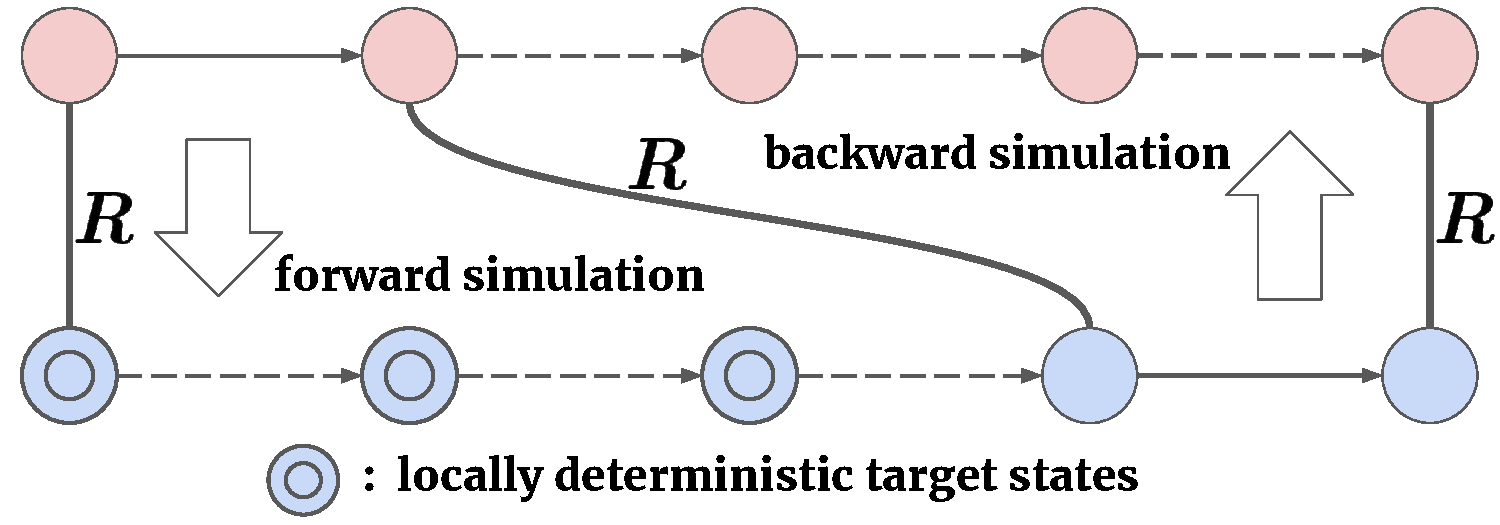
\includegraphics[width=0.7\textwidth]{images/mixed-sim-bold.pdf}
%% 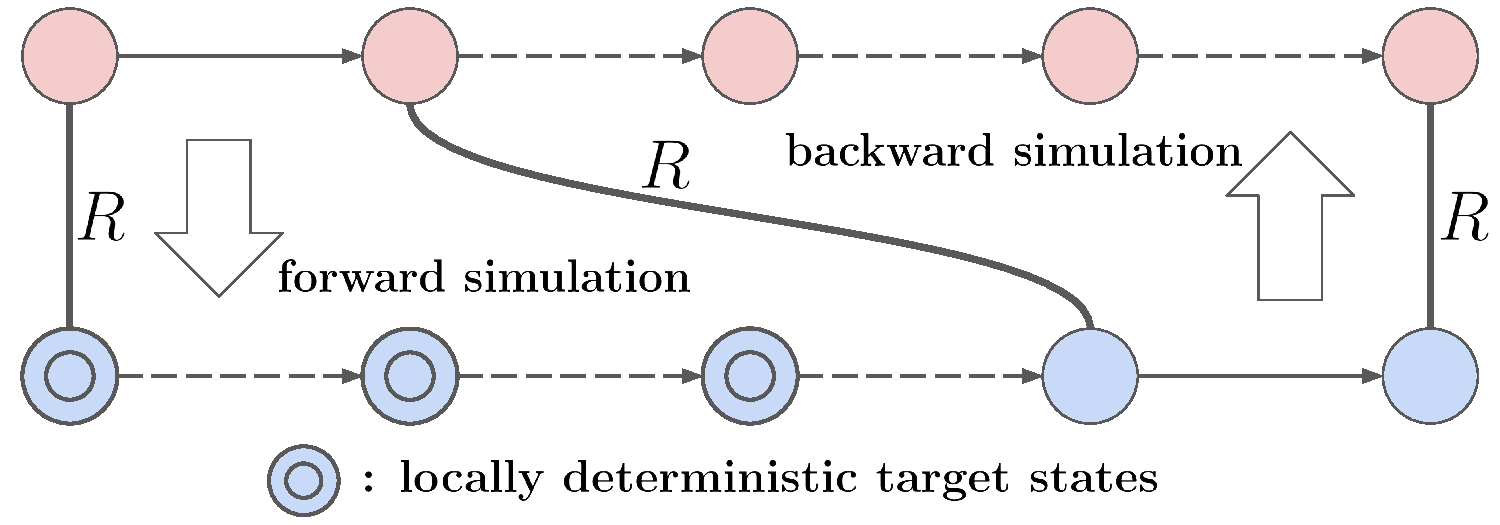
\includegraphics[width=0.7\textwidth]{images/mixed-sim.pdf}
\caption{A visualized example of mixed simulations}
\label{fig:mixedsim}
\end{figure}

\section{CompCertM}
\label{sec:compiler:compcertm}

Based on the theories we presented so far, we develop \ccm{}, an extension of \cc{} with the
repaired interaction semantics and open simulations to support multi-language linking.  We state
\ccm{}'s compositional correctness results (\Cref{sec:results:compiler}) and evaluate its
verification efforts (\Cref{sec:results:evaluation}).  \ccm{} currently supports the x86 backend only.
We do not currently see any technical problem with supporting other architectures.

\subsection{Compositional Correctness}
\label{sec:results:compiler}

\ccm{} uses open simulations with three parameters:
memory relations, symbol relations and memory predicates
(see \Cref{sec:main-verification:opensim} for details).
It supports $(i)$ the memory relations discussed in \Cref{sec:overview-verification:injection}:
identity, extension and (enriched) injections with no or any given module-local invariant;
$(ii)$ two symbol relations: one for keeping identical symbols in the source and target
and the other for allowing elimination of global variables in the target (only allowed for memory injections), needed for \code{Unusedglob} and \code{Unreadglob};
$(iii)$ two memory predicates: one for no analysis and the other for the value analysis of \cc{}.

Let $\rels$ be the set of open simulations with all possible parameters.
To apply RUSC, we prove that the \ccm{} compiler $\mathcal{C}$ transforms the source module with
a series of passes that are independently verified using open simulations in $\rels$.
\begin{lemma}[Pass Correctness]\label{thm:results-passes}
  For any \textrm{Clight} module $S$ and \textrm{Asm} module $T$, if $\mathcal{C}(S) = T$, then
  there exist intermediate modules $M_0, M_1, \cdots, M_n$ such that:
  \begin{enumerate}
  \item $M_0 = S$ and $M_n = T$; and
  \item $\forall i \in [0,n),~ \exists R \in \rels,~ (M_i, M_{i+1}) \in R$~.
  \end{enumerate}
\end{lemma}

We also prove all \textrm{Clight} and \textrm{Asm} modules are self-related.
\begin{lemma}[Self-Relatedness]\label{thm:results-relatedness} For any \textrm{Clight} or \textrm{Asm}
  module $M$, we have $M \in \self{\rels}$.
\end{lemma}
\noindent
\revision{Note that
  since we define illegal interference from Asm
  (\ie causing different behaviors in the source and target) as undefined behaviors (UBs)
  as shown in \Cref{sec:compiler:solution},
  every Asm module can be self-related.}

From \Cref{thm:results-passes,thm:results-relatedness}, the RUSC relation for the compiler follows.
\begin{theorem} [Modular Correctness]\label{thm:results-modular}
  For any \textrm{Clight} module $S$ and \textrm{Asm} module $T$, if $\mathcal{C}(S) = T$:
  \[
    {S} \rusc_\rels {T} \quad\text{with}\quad S,T \in \self{\rels}~.
  \]
\end{theorem}

\noindent
This theorem provides a truly compositional correctness
thanks to the compositionality of RUSC (\Cref{thm:rusc}):
%% The fact that the source and target are related by RUSC
%% implies that they satisfy behavioral refinement by adequacy of RUSC, and moreover
the relation can be freely (\ie vertically or horizontally) composed with any verification using RUSC
including that against mathematical specifications.
As an example, the following compositional correctness follows.
\begin{corollary} [Compositional Correctness 1]\label{thm:results-compiler}
  Let $(S_1,T_1), \ldots, (S_n,T_n)$ be pairs of source and target modules.
  If each pair is either compiled (\ie $\mathcal{C}(S_i) = T_i$ with $S_i$ \textrm{Clight} and $T_i$ \textrm{Asm}), or a self-related context (\ie $S_i = T_i \in \self{\rels}$), then
  \[
    \beh{S_1 \llink \cdots \llink S_n} \supseteq \beh{T_1 \llink \cdots \llink T_n}~.
  \]
\end{corollary}
%
\noindent This correctness theorem is compositional in the sense that behavior is refined in the
presence of any self-related contexts such as arbitrary \textrm{Clight} and \textrm{Asm} modules
(\Cref{thm:results-relatedness}).





Note that \textrm{Clight}, not \textrm{\cc{} C}, is the source language in the above theorems.  One of the
reasons is that \textrm{Clight} is the source language for most verification frameworks based on
\cc{}, such as VST~\cite{VST}, \ccc{}, and \ccx{}.  More importantly, we found that
\textrm{\cc{} C} is incompatible with memory injections.  Specifically,
\textrm{\cc{} C} imposes a strict alignment requirement on memory blocks of size zero, which, however,
%% but the requirement
is not preserved by memory injections.
%% For this reason, we cannot achieve full horizontal compositionality
%% in the presence of both \textrm{\cc{} C} modules and compiler passes verified using memory injections.
In other words, \textrm{\cc{} C} modules are not always self-related by memory injections.\footnote{This problem
  would be solved if one strengthens memory injections with more strict alignment requirements.}

\myparagraph{Supporting \textrm{\cc{} C}}
However, we can still prove a compositional correctness (not modular correctness as in \Cref{thm:results-modular}) for \textrm{\cc{} C}
following \scc{}'s \emph{Level A} technique~\cite{kang:scc},
which exploits the fact that all \textrm{CompCert C} modules are transformed to \textrm{Clight} modules
by the same two passes.
Specifically, the first pass is verified using an open simulation with the memory identity
and the second pass with memory injections, as done in the original \cc{}.
Then the following lemma follows from horizontal compositionality and adequacy of
open simulations (with memory identity and injection) and transitivity of behavioral refinement.

\begin{lemma} [ClightGen Correctness]\label{thm:results-clightgen}
  Let $(S_1,T_1), \ldots, (S_n,T_n)$ be pairs of source and target modules.
  If each pair is either translated (\ie $\textrm{ClightGen}(S_i) = T_i$ with $S_i$ \textrm{\cc{} C} and $T_i$ \textrm{Clight}), or a self-related context (\ie $S_i = T_i \in \self{\rels}$), then
  \[
    \beh{S_1 \llink \cdots \llink S_n} \supseteq \beh{T_1 \llink \cdots \llink T_n}~.
  \]
\end{lemma}



By composing \Cref{thm:results-compiler}, \Cref{thm:results-clightgen} and \Cref{thm:results-relatedness}, we have the following theorem.
\begin{theorem} [Compositional Correctness 2]\label{thm:results-compiler2}
  Let $(S_1,T_1), \ldots, (S_n,T_n)$ be pairs of source and target modules.
  If each pair is either compiled (\ie $\mathcal{C}(S_i) = T_i$ with $S_i$ \textrm{\cc{} C} or \textrm{Clight} and $T_i$ \textrm{Asm}), or a self-related context (\ie $S_i = T_i \in \self{\rels}$), then
  \[
    \beh{S_1 \llink \cdots \llink S_n} \supseteq \beh{T_1 \llink \cdots \llink T_n}~.
  \]
\end{theorem}


\myparagraph{Adequacy w.r.t. Physical Semantics}


We show that the repaired interaction semantics is adequate w.r.t. the physical semantics of \cc{},
where the former uses the language-independent linking $\llink$ and the latter the syntactic linking $\plink$
concatenating modules of the same language.

We prove that the physical semantics refines the repaired interaction semantics for \textrm{Asm} modules
using a closed simulation of \cc{} with memory injections.
\begin{theorem}[Adequacy w.r.t. Assembly]\label{thm:results-adequacy-asm}
  Let $M_1, \cdots, M_n$ be \textrm{Asm} modules.  We have:
  \[   \beh{M_1 \llink \ldots \llink M_n} \supseteq  \beh{M_1 \plink \ldots \plink M_n} ~.\]
\end{theorem}
\noindent
\revision{This theorem allows us to carry verification results on the interaction semantics such as \Cref{thm:results-compiler2}
down to \cc{}'s Asm semantics with syntactic linking.}



Conversely, we prove that the repaired interaction semantics refines the physical semantics for \textrm{\cc{} C} modules
using a closed simulation of \cc{} with memory identity.
This result is useful because we want to allow separate compilation (of C modules) on the compiler side, and on the program verification side, we want to hide complexities from inter-module steps.
\begin{theorem}[Adequacy w.r.t C]\label{thm:results-adequacy-c}
  Let $M_1, \cdots, M_n$ be \textrm{\cc{} C} modules.  We have:
  \[  \beh{M_1 \plink \ldots \plink M_n} \supseteq \beh{M_1 \llink \ldots \llink M_n}  ~.\]
\end{theorem}


In some sense, the \Cref{thm:results-compiler2,thm:results-adequacy-asm,thm:results-adequacy-c} together forms a strong stress-test for a language-independent linking, and our results show strong evidence that our repaired interaction semantics is indeed adequate (in a literal sense).
Specifically, if one of the three desiderata is missing, it is trivial to find language-independent linking satisfying the others.
Without \Cref{thm:results-adequacy-asm}, one can define interaction semantics to always execute UB; then, the other theorems become trivial.
Without \Cref{thm:results-adequacy-c}, one can define the behavior of interaction semantics to an empty set.
Without \Cref{thm:results-compiler2}, one can define $\llink \defeq \plink$.

%% These results mean that the repaired interaction semantics does not give too few behaviors to assembly programs (e.g., missing physically observable behaviors), nor does it give too many behaviors to well-typed C programs (e.g., giving UB to them).


Interestingly, by composing \Cref{thm:results-compiler2,thm:results-adequacy-asm,thm:results-adequacy-c}, we obtain
the same separate compilation correctness result of \scc{}~\cite{kang:scc}:

\begin{corollary}[Separate Compilation Correctness]
  Let $S_1, \ldots, S_n$ be \textrm{\cc{} C} modules and $T_1, \ldots, T_n$ be \textrm{Asm} modules.
  If $\mathcal{C}(S_i) = T_i$ for each $i$, we have:
  \[
    \beh{S_1 \plink \cdots \plink S_n} \supseteq \beh{T_1 \plink \cdots \plink T_n}~.
  \]
\end{corollary}

\youngju{Just mention that \ccc{} does not satisfy upperbound, and explain it in appendix?}
\youngju{here? or appendix?: To this end, we have strengthened \cc{}'s type checker in a number of
  ways, ruling out trivially wrong (according to C standard) programs more than before.  We rule out
  (i) a program that contains an identifier that is not declared in the module (ii) ``return''
  (without value) statement used for non-void function (iii) ``return'' (with value) statement used
  for void function (iv) function arguments containing void type.  (v) has duplicate (function or
  global variable) identifiers (vi) A function argument with size bigger than INT\_MAX (\cc{}
  already aborts on such programs)}





\subsection{Evaluation of Verification Efforts}\label{sec:results:evaluation}

\begin{table}[t]
\footnotesize

\parbox{\linewidth}{
\caption{SLOC of \ccm{} and related works --- compared to its baseline \cc{}, respectively}
\begin{tabu}{@{}l@{\hspace{1.55pt}}|[1.25pt]@{\hspace{1.55pt}} c @{\hspace{1.55pt}}|@{\hspace{1.55pt}} c @{\hspace{1.55pt}}|@{\hspace{1.55pt}} c @{\hspace{1.55pt}}|[1.25pt]@{\hspace{1.55pt}} c @{\hspace{1.55pt}}|@{\hspace{1.55pt}} c @{\hspace{1.55pt}}|[1.25pt]@{\hspace{1.55pt}}}
Portion     & \shortstack{\cc{} \\ 3.5} & \ccr{} 3.5        & \ccm{} pack                                               & \shortstack{\cc{}\\ 2.1} & \ccc{} \\
\hline
Pass Proofs & 34,376    & 35,893 (+4.41\%)  & \newrevision{4,923(+14.32\%)}                                          & 21,215    & 52,140 (+145.77\%) \\
The Rest    & 85,617    & 87,965 (+2.74\%)  & \newrevision{25,558(+29.85\%)}  & 59,365    & 107,910 \hspace{.6mm} (+81.77\%) \\
Total       & 119,993   & 123,858 (+3.22\%) & \newrevision{30,481(+25.40\%)}                                         & 80,580    & 160,050 \hspace{.6mm} (+98.62\%) \\
\end{tabu}
\\
\begin{tabu}{@{}l@{\hspace{1.55pt}}|[1.25pt]@{\hspace{1.55pt}} c @{\hspace{1.55pt}}|@{\hspace{1.55pt}} c @{\hspace{1.55pt}}|[1.25pt]@{\hspace{1.55pt}}}
Portion     & \shortstack{\cc{} \\ 3.0} & \ccx{}             \\
\hline
Pass Proofs & 26,466    & 30,572 (+15.51\%)  \\
The Rest    & 82,312    & 121,532 (+47.65\%) \\
Total       & 108,778   & 152,104 (+39.83\%) \\
\end{tabu}
\label{table:evaluation-ours}
}

%% \parbox{\linewidth}{
%% \label{table:evaluation-ours}
%% }
    
\parbox{0.38\linewidth}{
\vspace{4mm}
\caption{\mbox{Breakdown of \ccm{} pack}}
\begin{tabu}{@{}l | l@{}}
Portion                          & SLOC                                                                                                     \\
\hline
\revision{Proofs about Intermodule Steps} & \newrevision{4,923}                                                                                                    \\
Interaction Semantics/Properties & 1,940                                                                                                    \\
Language Semantics/Properties    & 1,701                                                                                                    \\
Self Simulations                 & \newrevision{5,593}                                                                                                    \\
\cc{}  Metatheory Extension      & \newrevision{4,688}                                                                                                    \\
\ccm{} Metatheory                & \newrevision{7,656}                                                                                                    \\
Mixed Simulation                 & 1,090                                                                                                    \\
Adequacy w.r.t. Asm              & 2,890                                                                                                    \\
\end{tabu}
\label{table:evaluation-breakdown}
}
\hfill
\parbox{0.45\linewidth}{
\vspace{4mm}
\caption{SLOC of additional developments}
%% \begin{tabu}{@{}l @{\;} |[1.25pt] @{\;} r @{\;} | @{\;} r @{\;} | @{\;} r @{\;} | @{\;} r @{\;} | @{\;} r @{}}
%% Portion                          & \shortstack{\texttt{Unreadglob} \\ 3.5} & \shortstack{\texttt{Unreadglob} \\ pack} & \texttt{mutual-sum} & \texttt{utod} & \shortstack{Adequacy \\ w.r.t. C} \\
%% \hline
%% Pass Proofs                      & 1,842                   & 338                      & 3,088               & 361           & -             \\
%% The Rest                         & 260                     & 1,933                    & 2,707               & 424           & 4,044         \\
%% Total                            & 2,102                   & 2,271                    & 5,795               & 785           & 4,044         \\
%% \end{tabu}
\begin{tabu}{@{}l @{\;} |[1.25pt] @{\;} r @{\;} | @{\;} r @{\;} | @{\;} r @{\;} | @{\;} r @{\;} | @{\;} r @{}}
Portion                          & \shortstack{\texttt{Unreadglob} \\ 3.5} & \shortstack{\texttt{Unreadglob} \\ pack} & \shortstack{Adequacy \\ w.r.t. C} \\
\hline
Pass Proofs                      & 1,842                   & 338                      & -             \\
The Rest                         & 260                     & 1,933                    & 4,044         \\
Total                            & 2,102                   & 2,271                    & 4,044         \\
\end{tabu}
\label{table:evaluation-others}
}%
\end{table}

\youngju{There are two ``unreadglob'' columns, one for \cc{} and one for pack. Simplify it}
\youngju{How about reducing caption text size?}
\jeehoon{``Per-pass'', ``Metatheory'', and ``Total'' instead of ``Pass Proofs'', ``The Rest'', and ``Whole''}

To demonstrate that \ccm{} is lightweight,
we compare significant lines of code (SLOC) of \ccm{}, \ccc{}, and \ccx{} with
those of their baseline \cc{} versions 3.5, 2.1, and 3.0, respectively.
Overall, \ccm{} adds less code to \cc{} than \ccc{} and \ccx{} do,
and in particular significantly less code than \ccc{} for the proofs of compiler passes.%
\footnote{\revision{Note that \ccc{} allows horizontal compositionality between any intermediate languages (ILs)
  while \ccm{} only between Clight and Asm since self-relatedness is proven only for the two.
  Though practically unnecessary, supporting linking between arbitrary ILs in \ccm{} would increase SLOC to prove self-relatedness for the other ILs.}}
\newrevision{Also note that \ccr{} uses the enriched memory injections of \Cref{sec:overview-verification:injection:dynamic} instead of the original memory injections
in order to give reusable main lemmas for both closed and open simulations.
Since \ccr{}'s pass proofs are only 4.41\% larger than \cc{}'s, 
the overhead due to handling the private memory components of enriched memory injections is, roughly speaking, at most 4.41\%.}

\Cref{table:evaluation-ours} summarizes the comparison.
For each compiler (\ie each column),
the rows report SLOC for the proofs of all compiler passes (Pass Proofs),
the rest of the development (The Rest),
and their summation (Total).
Note that \ccm{} is split into \ccr{} and \ccm{} pack, for which the former is our refactoring
of \cc{} and the latter is an additional package to support multi-language linking.
We counted SLOC reported by
\code{coqwc}.\footnote{Concretely, we counted ``spec'' and ``proof'' lines reported by \code{coqwc}.
  Because we use a different criteria for line numbers, they are different from those reported in
  prior work~\cite{stewart:ccc,gu:dscal,wang:saccx}.}  When counting SLOC, we excluded the following
code for fair comparison: $(i)$ code for other architectures than x86 because all three projects support
only x86; $(ii)$ code for the parser and type checker introduced in later versions of \cc{}; and $(iii)$ code for \textrm{ClightGen}, which is not supported by both \ccx{} and
\ccc{}.  We also excluded \ccc{}'s legacy proofs for the original compiler correctness.  We used the
latest development branches for the three projects.\footnote{Development as of November 8, 2019, available at: \url{https://github.com/snu-sf/compcertr}, \url{https://github.com/snu-sf/compcertm}, \url{https://github.com/PrincetonUniversity/compcomp}, \url{https://github.com/DeepSpec/dsss17/tree/master/CAL}}








\Cref{table:evaluation-breakdown} analyzes the \newrevision{30,481} SLOC for \ccm{} pack.
\revision{The pass proofs consist of \newrevision{4,923} SLOC for reasoning about intermodule steps, which is
  sometimes nontrivial since they perform the logical instrumentation presented in \Cref{sec:compiler:solution}.
  Note that \ccr{} provides proofs for intramodule steps as main lemmas, which are reused in \ccm{}.
}
The rest consists of
1,940 SLOC for the repaired interaction semantics and its properties;
1,701 SLOC for properties of each language such as determinism and receptiveness;
5,576 SLOC for self-relatedness (\Cref{thm:results-relatedness});
4,687 SLOC for extending the metatheory of CompCert;
7,569 SLOC for open simulations and other metatheory for \ccm{};
1,090 SLOC for mixed simulation; and
2,890 SLOC for adequacy w.r.t. assembly (\Cref{thm:results-adequacy-asm}).

%% \Cref{table:evaluation-others} shows SLOC for the new optimization pass and the verification examples
%% given in the dissertation.  Note that \code{Unreadglob} 3.5 adds the optimization to \ccr{} proving closed simulation
%% and \code{Unreadglob} pack to \ccm{} proving open simulation, which reuses the proof of \code{Unreadglob} 3.5 for intramodule steps.
%% As the verification of \code{mutual-sum} and \code{utod} show, directly proving
%% open simulation between programs and specifications is costly. 
%% We believe that program logics like VST~\cite{VST} can be used to prove such simulation,
%% which could significantly reduce the verification cost.
\Cref{table:evaluation-others} shows SLOC for the new optimization pass.  Note that \code{Unreadglob} 3.5 adds the optimization to \ccr{} proving closed simulation
and \code{Unreadglob} pack to \ccm{} proving open simulation, which reuses the proof of \code{Unreadglob} 3.5 for intramodule steps.


\section{Formal Semantics}
\label{sec:compiler:semantics}
abc

\section{Formalization of Verification Techniques}
\label{sec:compiler:verification}
abc

\section{Related Work}
\label{sec:compiler:related}
abc

%% \input{unsoundall}
Compiler rightfully assumes two properties about its context (\ie{} assemblies that could be linked with) and exploit it in its translation.
First, compiler assumes \textit{callee-save registers} to remain the same across a function call.
This property is vital for compiler performance, because without this assumption a compiler should always spill its data into memory whenever it encounters a call to external function.
Second, compiler assumes a variable that is not leaked, \ie{} \textit{private}, to be unchanged across during a function call.
A simple example showing the how compiler uses this assumption is \Cref{fig:compiler}.
Constant propagation, one of the most important optimization, translates (a) into (b) assuming *x it is not changed.

However, an arbitrary assembly may break these properties.
First property could easily be broken if \code{g} writes to a callee-save register without recovering it.
Suppose (a) is compiled to an assembly where \code{x} is stored in a callee-save register, say \code{\%rbx}.
If it is linked with (c), \code{f} will return 1.
Second property could also be broken and one possible reason is illegal access to the data passed in callee-save register. %% another reason: guessing. idsim prevents it
Similarly, if \Cref{fig:unsoundall}-(a) linked with (b) it will return 1.

This is an essential problem when defining a general multi-language semantics, regardless of how we define semantics.
We stress \textit{general} here to note that previous works such as \scc{} and \ccx{} were free from this problem.
This is because they were interested only in a restricted set of well-formed assemblies (compiler-generated assemblies and assemblies proven to satisfy so called \textit{primitive specification}, respectively).

In order to define a sound semantics, we should give \textit{undefined behavior} to such ill-behaved assembly, precisely.
Undefined behavior can be understood as a tool to exclude ill-behaved program from reasoning in a \textit{semantic} way.
Mathematically, undefined behavior is a set of all behaviors.
\todo{explain it - enables refinement, disables verification}


%% Mathematically, undefined behavior is a set of all behaviors.
%% By giving undefined behavior to an ill-behaved program, we can attain \textit{soundness} of our semantics: \ie{} the semantics validates compiler optimizations and actual behavior refines behavior given by the semantics.

%% We want our semantics to support general.
%% Instead of syntactically quantifying, semantically quantifying precisely. ---> difference between CCX?

\myparagraph{Semantics (tentative)}
Similar to \ccc{}, we build multi-language semantics by instantiating interaction semantics but with substantially different ingredients.
Before we proceed, we will briefly explain interaction semantics.

Intuitively, the idea behind interaction semantics is to model multi-language semantics by gluing together each languages’ existing semantics, while considering them as a black box.
To this end, whenever a function of a language, say, $L$ is called, a state of type $L.(state)$ is spawned and dedicated.
As a consequence, the behavior of that function can be described solely by reusing $L$'s semantics, considering only its dedicated state and ignoring an outside world.

A problem with \ccc{} was that it was unsound, as the first property was not enforced.
As mentioned above, the actual behavior of \Cref{fig:unsoundall} is returning 1, as there is one, shared register set.
However, in interaction semantics, each function has its own state, (register set, here).
As a consequence, b.s modifies \textit{its} \code{\%rbx} and it does not affect that of a.s.
Therefore, \ccc{}'s semantics will confidently say that it returns 0.

In order to address this discrepancy, it is crucial to enforce the calling convention somehow.
In other words, if some callee-save register has a different value between the beginning and the end of a function, it should be \textit{undefined behavior}.
This discovery leads us to the next question: what should be the initial value of such a callee-save register?
In \ccc{}, it is an undef value.
This is an appropriate choice because its actual value on runtime could differ arbitrarily by its caller.
%% Why not zero?
However, adding one to undef value still results in undef value.
Therefore, it does not trigger undefined behavior and the problem is unresolved.
Note that whatever value you chose (\eg{} 0) to initialize \code{\%ebx}, I can modify \code{\%rbx + 1} into the value of your choice, and the problem remains the same.

One naive fix is to initialize it dynamically with the value of the caller's register, instead of a statically fixed one, but it still does not work.
In that case, examples above will properly give undefined behavior.
However, recall that we are defining a multi-language semantics: what if the caller is a C function?
We cannot foresee what caller's register's value will be, as we do not know how the caller will be compiled: the semantics should be sound no matter which compiler and optimizations we use.

%% We argue that the flaw of this game lies in \textit{determinism}.
We argue that the root cause of this problem is \textit{determinism}.
Our solution is to initialize each register with an arbitrary value, in a \textit{nondeterministic} way.
By doing so, if there is a single choice of value that causes callee-save checking to fail, it is undefined behavior.
That is, we are effectively enforcing calling convention to be satisfied \textit{no matter what values} are passed in callee-save registers.

However, full nondeterminism breaks the second property.
\todo{}



\myparagraph{Proof (tentative)}
\todo{mixed simulation}



-----------------------------------------------------------------
-----------------------------------------------------------------
-----------------------------------------------------------------
-----------------------------------------------------------------
-----------------------------------------------------------------
-----------------------------------------------------------------
-----------------------------------------------------------------
-----------------------------------------------------------------
-----------------------------------------------------------------
-----------------------------------------------------------------
-----------------------------------------------------------------

Consider the following example: \Cref{fig:compiler}-(c).
Here, \code{y} is introduced just to forbid constant propagation.
In its final target, \code{y} will be stored in a callee-save register and
\Eg{} a compiler will translate \Cref{fig:compiler} a compiler will assign a callee-save register for the variable \code{x}, and


and a sound semantics should give undefined behavior on such assembly.
Basically, Callee-save registers


This is an unavoidable



Similar to \ccc{}, we build multi-language semantics by instantiating interaction semantics, but with substantially different ingredients.

Compiler rightfully assumes callee-save registers remain the same across a function call, but arbitrary assembly code may break this property.
- this is an essential challenge
- in \scc{}, there was no problem

In \ccc{}, defined it with undef, but it is not sound


The last

\myparagraph{Interaction Semantics}

\myparagraph{Memory (tentative)}



%% introduced and then by will describe why \ccc{}'s semantics fails to satisfy desiderata, and lead you to our solution step by step.
%% Similar to \ccc{}, we build multi-language semantics by instantiating interaction semantics, but with substantially different ingredients.

Similar to \ccc{}, we build multi-language semantics by instantiating interaction semantics, but with substantially different ingredients.
\myparagraph{Interaction Semantics}
Intuitively, the idea behind interaction semantics is to model multi-language semantics by gluing together each languages’ existing semantics, while considering them as a black box.
To this end, whenever a function of a language, say, $L$ is called, a state of type $L.(state)$ is spawned and dedicated.
As a consequence, the behavior of that function can be described solely by reusing $L$'s semantics, considering only its dedicated state and ignoring an outside world.

%% \input{unsoundall}
\myparagraph{Callee-save Checking}











\ccc{}'s semantics is unsound as it is not \lbound{}, and the key ingredient to address this problem is nondeterminism.

%% Consider this example \Cref{fig:unsoundall}.
\Cref{fig:unsoundall} shows why \ccc{} is not \lbound{}.
Note that these are assembly programs: we used C syntax just for readability.
When the \code{main} is linked with (a) and ran in actual CPU, it will obviously print 2.
Nonetheless, according to \ccc{}'s semantics, it prints 1!
As explained, in interaction semantics, each function call is dedicated its own state (register set, here), while in reality there is one, shared register set.
%% Take this setting for granted, caller expects its callee-save registers to remain the same across the function call.
%% \input{unsound}
The caller (main) rightfully assumes its callee-save registers to remain the same across the function call, but the callee (f) breaks the \textit{calling convention}.
In order to address this discrepancy, it is crucial to enforce the calling convention. %% on each function.
In other words, if some callee-save register has a different value between the beginning and the end of a function, it should be \textit{undefined behavior}.

This discovery leads us to the next question: what should be the initial value of such a callee-save register?
In \ccc{}, it is \textit{undef}.
This is an appropriate choice because its actual value on runtime could differ arbitrarily by its caller. %% it is impossible for callee to expect any specific value in the register. %% to know which context will call the function.
%% However, now consider the example on the right (\Cref{fig:unsound2}).
However, now suppose the \code{main} is linked with (b).
According to our slightly modified semantics (that checks if callee-save registers remain the same), \code{f} passes the checking, and it still prints 1.
Note that whatever value you chose (\eg{} 0) to initialize \code{\%ebx}, I can modify \code{INTMAX + 1} of \code{f} into the value of your choice, and the problem remains the same.

One naive fix is to initialize it dynamically with the value of the caller's register, instead of a statically fixed one, but it still does not work.
In that case, examples above will properly give undefined behavior.
However, recall that we are defining a multi-language semantics: what if the caller is a C function?
We cannot foresee what caller's register's value will be, as we do not know how the caller will be compiled: the semantics should be sound no matter which compiler and optimizations we use.

%% We argue that the flaw of this game lies in \textit{determinism}.
We argue that the root cause of this problem is \textit{determinism}.
Our solution is to initialize each register with an arbitrary value, in a \textit{nondeterministic} way.
By doing so, if there is a single choice of value that causes callee-save checking to fail, it is undefined behavior.
That is, we are effectively enforcing calling convention to be satisfied \textit{no matter what values} are passed in callee-save registers.




\myparagraph{Junk Pointers}

Nonetheless, the problem is not over yet: so far, we have only considered lower bound proof, but compiler correctness proof complicates the problem once again.
\todo{specifically, self simulation of assembly}
\todo{For efficiency ? we want our semantics to satisfy the following three constraints}.
First, \todo{initial state is injected}
\todo{explain \cc{} injection? where?}
\todo{1. it is more efficient 2. to reason arbitrary assembly. if not-injected, passing it to extcall will break reasoning}
Second, \todo{src callee-save checking succeeds -> tgt succeeds}
\todo{1. it is more efficient}
\todo{2. to reason in modular way. f := x = g(); --> src checking succeeds (U-U) tgt checking fails (0-1)}
Third, \todo{we want to allow pointer arithmetic?}

Naive nondeterminism fails to satisfy these constraints.
%% Naive nondeterminism fails.
\todo{\cc{} injection has target private pointer, the only value that injects it is undef}
\todo{src begins with undef -> second property fails}

Therefore, we developed a novel trick called \textit{junk pointer} to address this problem.
\todo{explain junk pointer and proof strategy for self sim and lower bound}





















\myparagraph{Memory}








\section{Overview}\label{sec:overview}
In this section, we show an outline of our development, key ideas of our semantics and proof technique, motivating each one by comparing with \ccc{}.

\subsection{Development Outline}\label{sec:overview:outline}
%% \todo{we will explain why our strategy is extensible in both axis}


\myparagraph{Compositional Compiler Correctness}
\ccc{}'s proof strategy is modular, but only to some extent.%% , but ours is entirely modular.
\ccc{} is modular in the sense that it proves each translation separately.
However, the simulation relation it uses is globally fixed to a \textit{single} one which is sophisticated enough to reason every pass, which currently is structured injection.
So this breaks modularity: even a trivial translation using the simplest relation is \textit{enforced} to be reimplemented to use structured injection, because of compositionality with \textit{other} translations.
Moreover, suppose that future \cc{} has introduced a translation that is too complex for structured injection to reason with.
Then, this introduction of a single pass breaks whole proof: the \textit{single} relation should be adjusted to cover it, and every existing proof should be updated accordingly.

Our proof strategy is entirely modular, and the key distinction is that we do not require vertical compositionality of \textit{simulation relation}.
\ccc{} relied on vertical compositionality of simulation relation, which is known to be a notoriously hard problem.
Not to mention its proof, a question whether such relation composes is a surprisingly nontrivial problem, and finding appropriate relation is itself an interesting research problem. \cite{TODO}
In \ccc{} context, proving vertical compositionality at least required a nontrivial amount of development: the proof is 5274 SLOC long, and it enforced to re-implement each language's semantics with effect annotations.
The problem gets more complicated if we consider multiple different relations, and we believe that is the reason why Stewart \etal{} fixed a single simulation relation. %% to avoid proving vertical compositionality as much as possible.
%% A. Ahmed, D. Dreyer, and A. Rossberg, “State-dependent representationindependence,” inPOPL, 2009
%% D. Dreyer, G. Neis, and L. Birkedal, “The impact of higher-order stateand  control  effects  on  local  relational  reasoning,”J.  Funct.  Program.,vol. 22, no. 4-5, pp. 477–528, 2012.
In contrast, as we do not require vertical compositionality of simulation relation, we are free from such problems and obtain \textit{true modularity}: each translation can choose the simulation relation of its interest.
%% Stewart \etal{} rather fixed a \textit{single, most sophisticated} simulation relation for whole translation proof.



%% \begin{wrapfigure}{R}{.4\textwidth}
\begin{figure}
  \centering
  %% 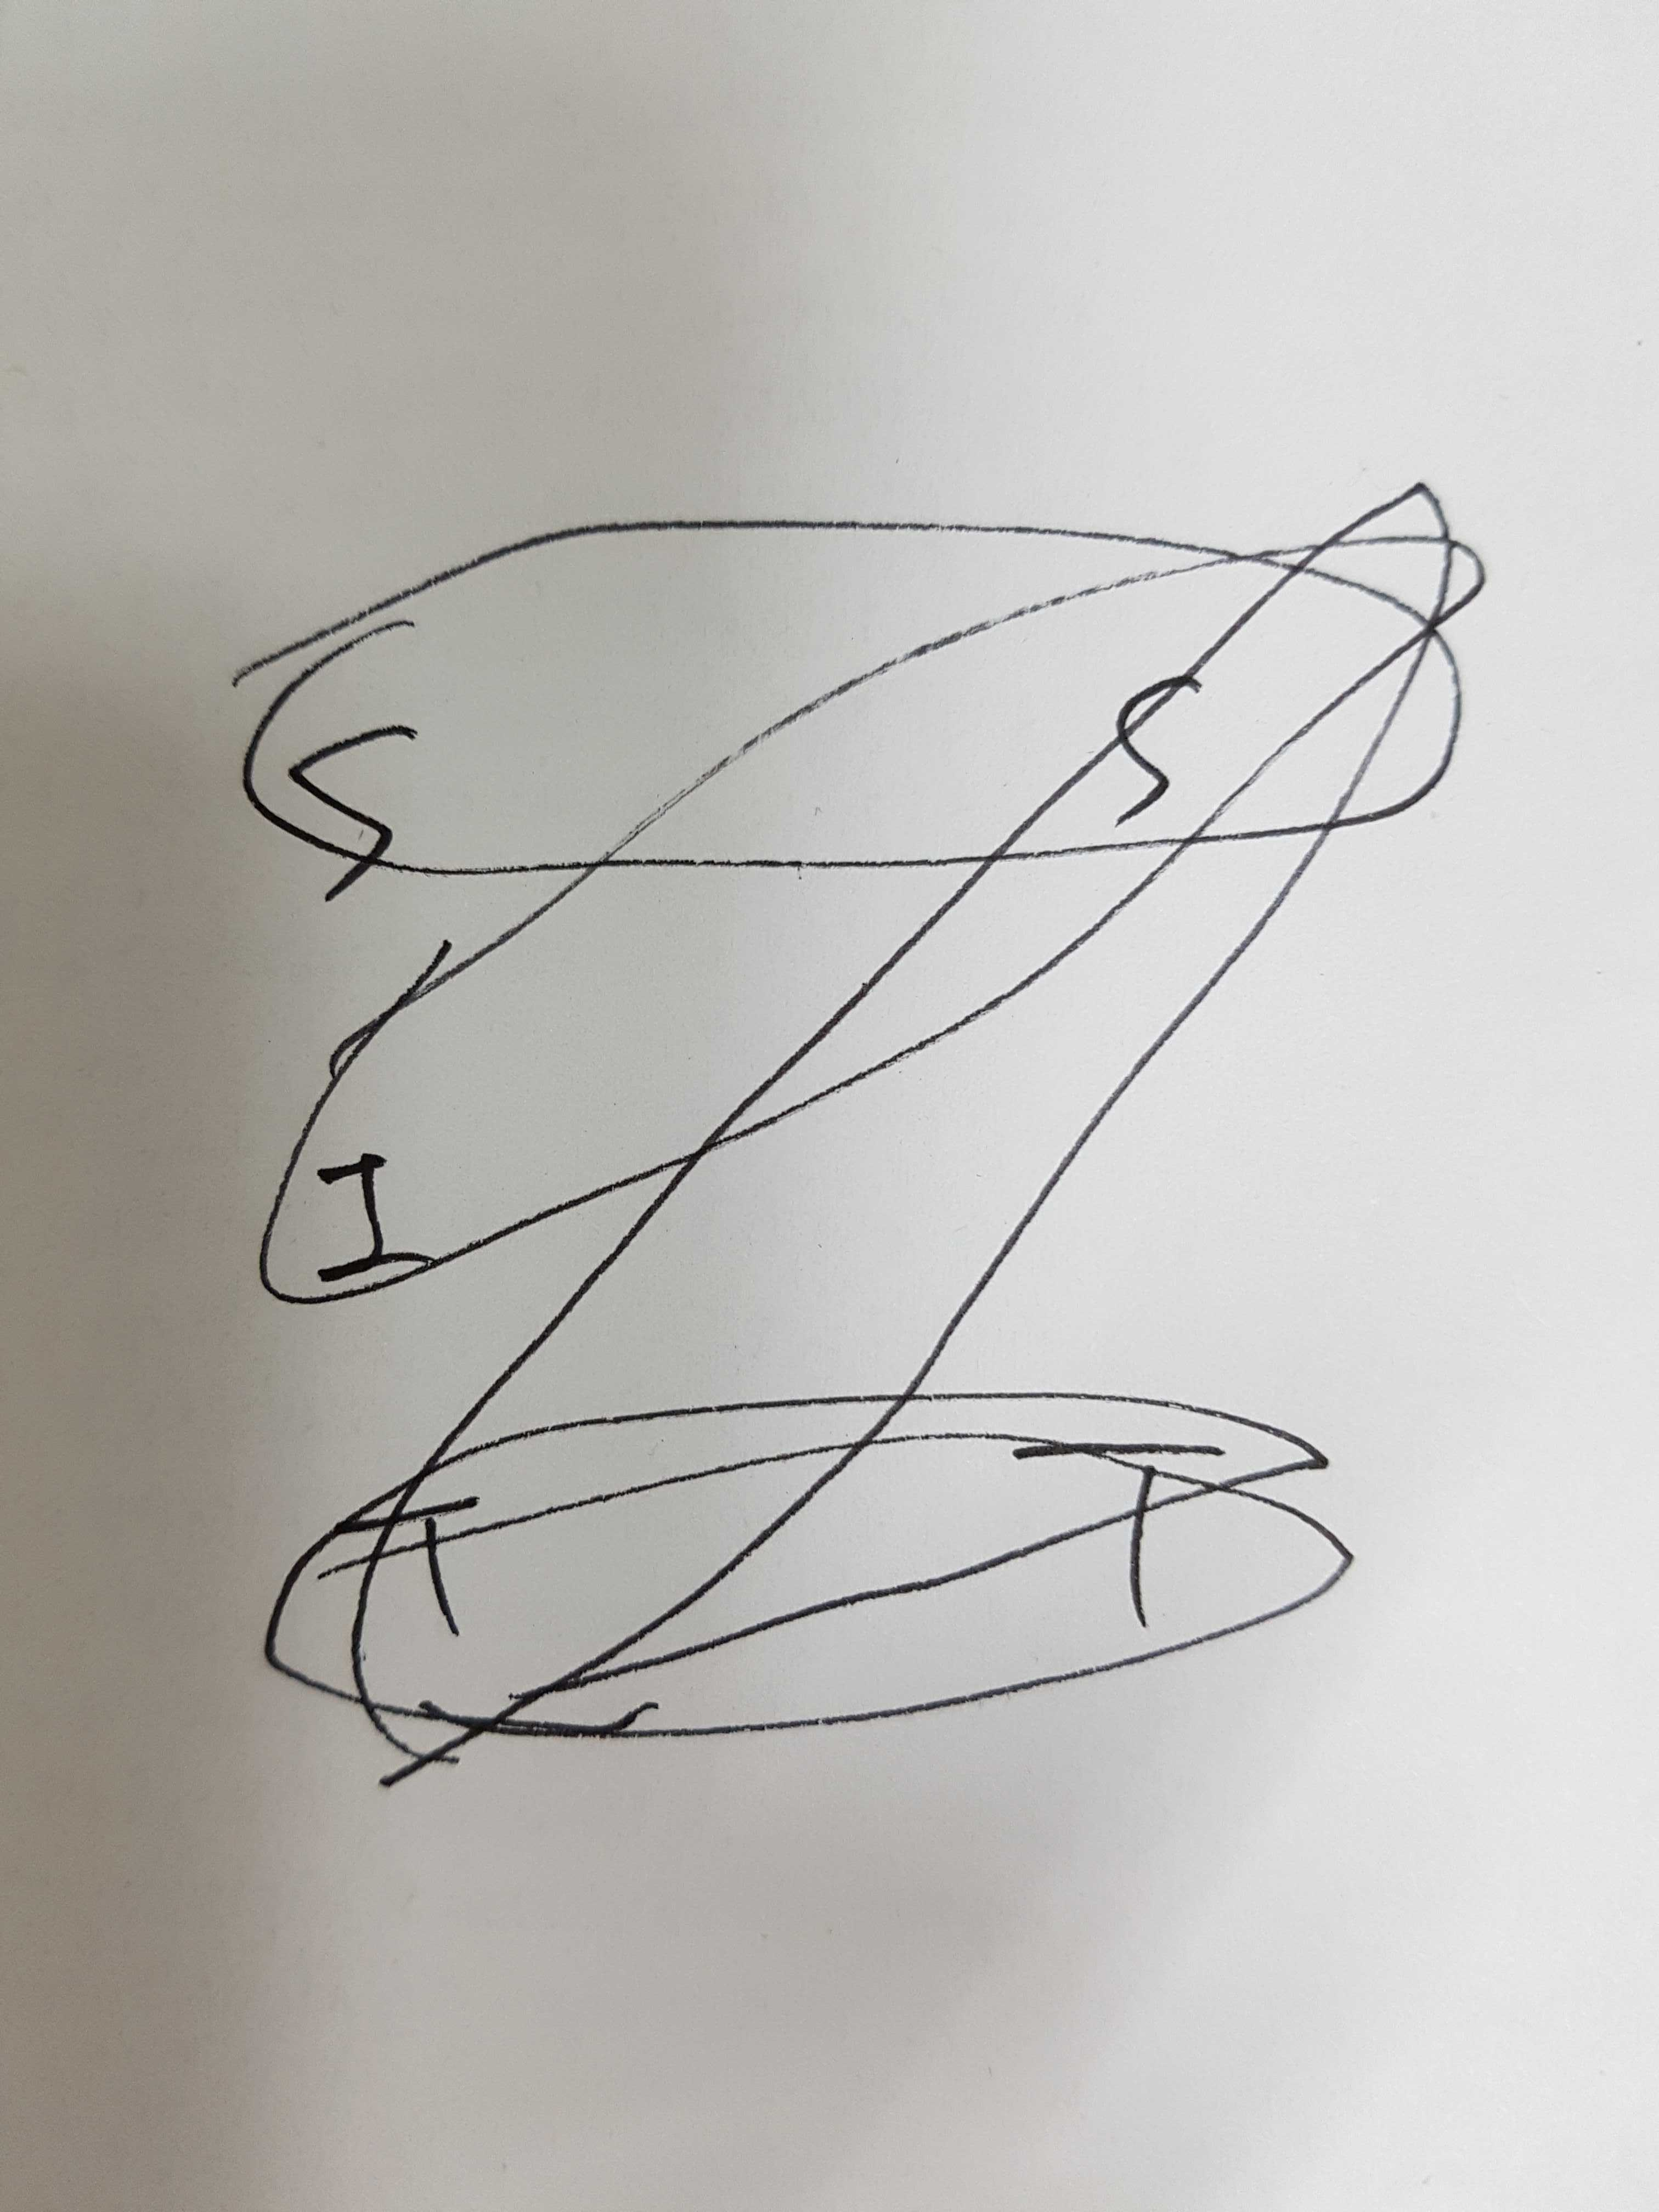
\includegraphics[width=1.0\linewidth]{images/draft-fig.jpg}
  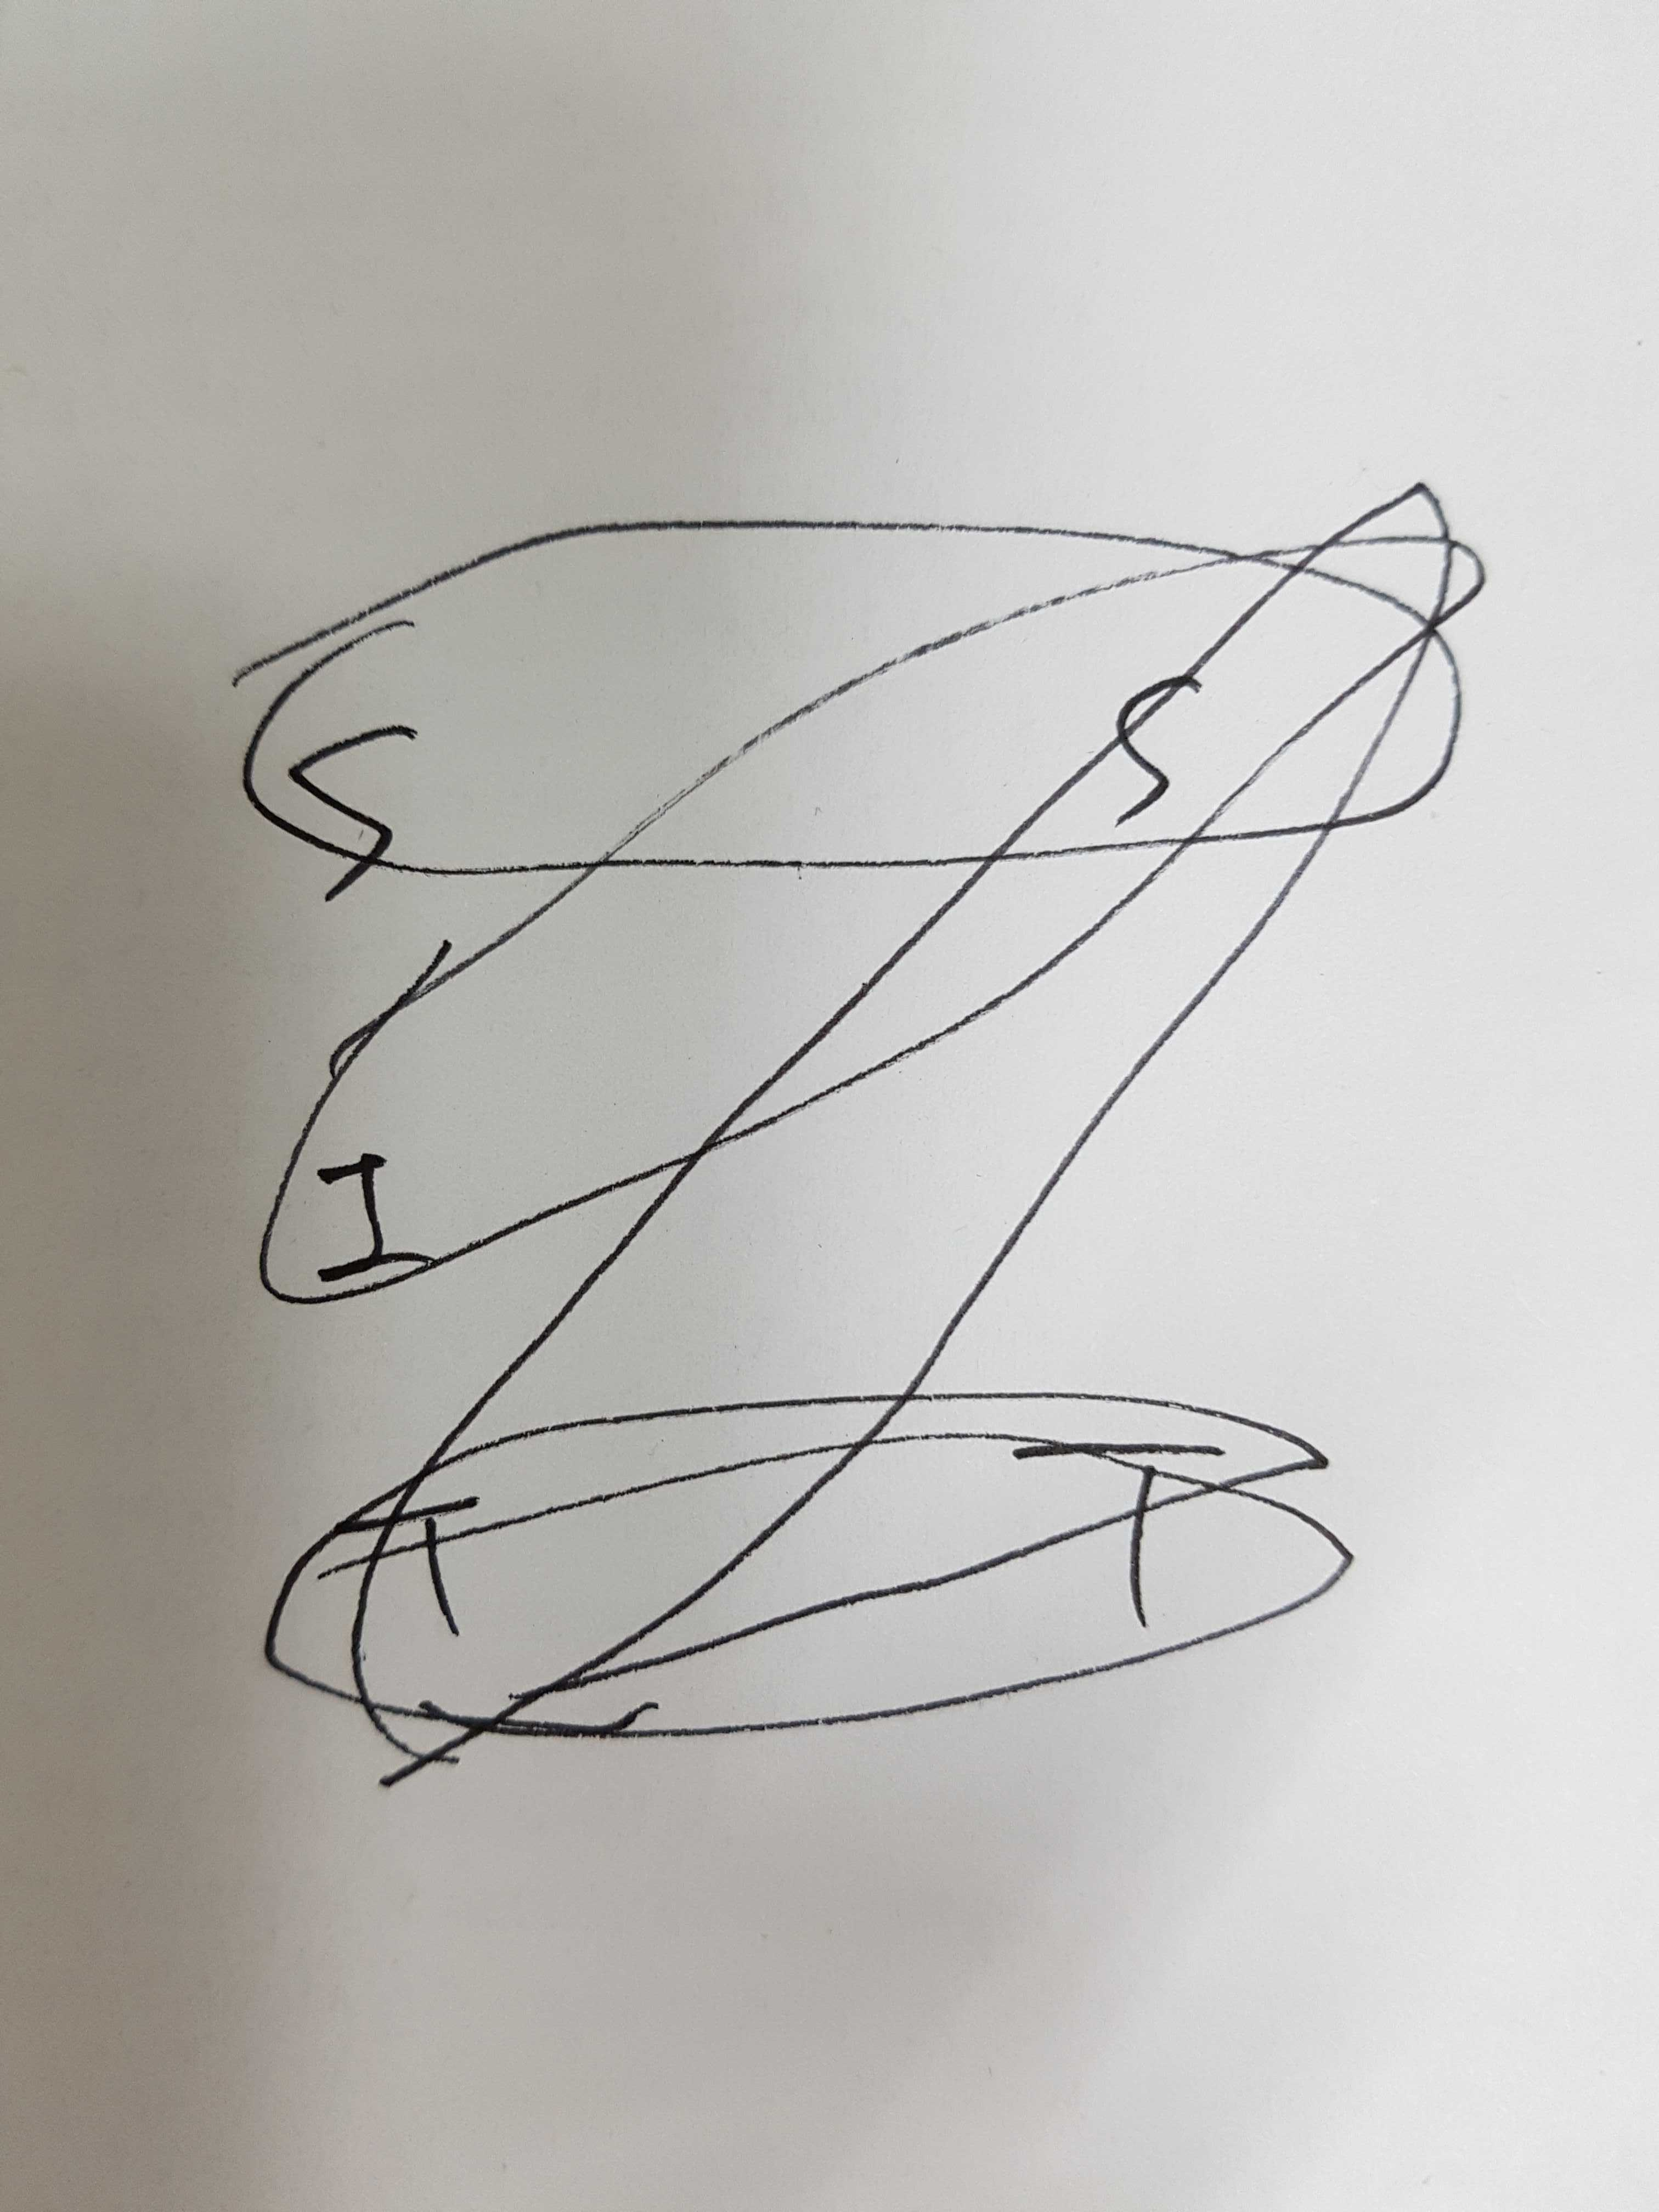
\includegraphics[width=0.35\linewidth]{images/draft-fig.jpg}
  \caption{
  }
  \label{fig:draft-fig}
\end{figure}
%% \end{wrapfigure}

We avoid proving vertical compositionality of \textit{simulation relation}, and instead, we compose in \textit{behavior} level, which is made possible because we are defining multi-language semantics.
\todo{compare with PILS - it is not multi-language semantics}
\todo{compare with Amal Ahmed? Their contextual equivalence is not modular}
%% But since all the languages in the compiler pipeline are taken into account when verifying each pass, this is far less modular than vertical compositionality.


\todo{Add simplified formalizations here? or later?}


Our proof strategy does not require such; each translation can chose whatever relation (in other words, rely and guarantee conditions) it wants.
The key distinction that leads to such difference is that we do not require vertical compositionality of \textit{simulation relation}, instead we compose in \textit{behavior} level.
Note that proving vertical compositionality is a notoriously hard work \cite{TODO}. %%pilsner?
Therefore, in order to avoid such complexity as much as possible, Stewart \etal{} rather fixed a \textit{single, most sophisticated} simulation relation for whole translation proof.

However, it is practically important to allow different simulation relation for each translation passes.
%% Note that vanilla \cc{} uses three different simulation relations, and porting it \todo{costed a lot}.
We will discuss this more in \cite{sec:overview:proof}.
Second, also, in order to prove vertical compositionality, they had to annotate each language's semantics with memory effects.


\ccc{} relies on vertical compositionality of simulation relation which harms true modularity.
In contrast, we compose in \textit{behavior} level, which is as simple as transitivity of set inclusion.

%% Like \ccc{}, we verify compiler correctness in a \textit{modular} way.
%% However, a little tweak here grants us significant benefit at the cost of proving a trivial fact.


%% but is little different, having significant benefit at the cost of proving a trivial fact.
%% Different from that of \ccc{}, our proof strategy has significant benefit at the cost of proving a trivial fact.





%% \subsection{Bounding Semantics}
\myparagraph{Lower Bound}
Lower bound is a part of soundness condition that multi-language semantics should satisfy, stating its behavior should at least contain \textit{actual behavior}.
It is formalized as follows.
%% Informally speaking, we want the behavior of multi-language semantics to at least contain an actual behavior when ran on a machine.
%% This property is a part of soundness of a semantics, and breaking it equals collapse of whole verification stack.
%% We have named this property as being \textit{bounded below} or \textit{lower bound}, and formalized it as follows.

\begin{theorem} (Lower bound)
  \[
  %% \forall \, A_{1} \, \ldots \, A_{n}, \,
  \mathcal{B}(L(A_{1}, \ldots, A_{n})) \supseteq \mathcal{B}(\llbracket A_{1} \circ \ldots \circ A_{n} \rrbracket)
  \]
\end{theorem}

\todo{explain $\circ$ notation and physical linking}

Then, together with compiler correctness proof, \todo{clarify it before} we can assure verification done in source level holds in actual behavior.
Note that we did not choose target arbitrarily: a syntactically linked assembly program is the current final target of \cc{}.
In other words, it is trusted computing base of \cc{} that syntactically linked assembly program properly models actual behavior, and we do not add any assumption.


\myparagraph{Upper Bound}
Upper bound is the dual of lower bound, and formalized as follows.
Although this property is not as vital as lower bound - it is not related to soundness - it is desirable for three reasons.
We require each C modules to be type\mymathhyphen{}checked for a technical reason which will be addressed in \Cref{sec:overview:semantics}

\begin{theorem} (Upper bound)
  \[
  %% \forall \, C_{1} \, \ldots \, C_{n}, \,
  C_{1}, \ldots, C_{n}, \, (C_{1} \circ \ldots \circ C_{n}) \; are \; type-checked \implies
  \mathcal{B}(\llbracket C_{1} \circ \ldots \circ C_{n} \rrbracket) \supseteq \mathcal{B}(L(C_{1}, \ldots, C_{n}))
  \]
\end{theorem}

First, this is a strong stress test for usability.
Note that both lower bound and compiler correctness proof becomes trivial if we define our semantics to be always undefined behavior, \ie{} set of all behaviors.
However, such semantics is not at all useful for user: one cannot verify anything with it.
Therefore, We would like to have a theorem that assures we didn't do such a thing.
Our formalization is the most sensible and strong such theorem we can think of.

Second, by composing with compiler correctness and lower bound theorem, we can get the correctness of separate compilation for free.
\todo{we support different version of \cc{}, while \scc{} cannot}
\begin{corollary} (Separate compilation correctness)
  \[                            %
  C_{1}, \ldots, C_{n}, \, (C_{1} \circ \ldots \circ C_{n}) \; are \; type\mymathhyphen{}checked \implies
  \mathcal{B}(\llbracket C_{1} \circ \ldots \circ C_{n} \rrbracket) \supseteq \mathcal{B}(\llbracket \mathcal{C}(C_{1}) \circ \ldots \circ \mathcal{C}(C_{n}) \rrbracket)
  \]
\end{corollary}
\begin{proof}
  TODO
\end{proof}
Finally, it can help reasoning and verification by hiding details of intermodule protocols.
\ie{} we want to allow users to reason about separately compiled C modules as if they were one.
%% Furthermore, with slight modification, we can get stronger theorem which allows input program to contain assembly.
To this end, instead of proving upper bound directly, we prove the following two lemmas which together imply upper bound.
Contrary to the aforementioned upper bound theorem, upper bound compression lemma can be used where source program contains assembly.

%% \todo{consequently, allow user to reason in syntactically linked program, bypassing meta-level call},
%% \todo{we assume all C modules here are type-checked for technical reason}

\begin{lemma} (Upper bound compression)
  \[
  %% \forall \, C_{1} \, C_{2} \, ctx, \,
  C_{1}, \ldots, C_{n}, \, (C_{1} \circ \ldots \circ C_{n}) \; are \; type\mymathhyphen{}checked \implies
  \mathcal{B}(L(ctx, (C_{1} \circ \ldots \circ C_{n}))) \supseteq \mathcal{B}(L(ctx, C_{1}, \ldots, C_{n}))
  \]
\end{lemma}

\begin{lemma} (Upper bound lifting)
  \[
  %% \forall \, C, \,
  C \; is \; type\mymathhyphen{}checked \implies
  \mathcal{B}(\llbracket C \rrbracket) \supseteq \mathcal{B}(L(C))
  \]
\end{lemma}





\subsection{Semantics}\label{sec:overview:semantics}
Similar to \ccc{}, we build multi-language semantics by instantiating interaction semantics, but with substantially different ingredients.
In this subsection, we will describe why \ccc{}'s semantics fails to satisfy desiderata, and lead you to our solution step by step.

\myparagraph{Interaction Semantics}
Intuitively, the idea behind interaction semantics is to model multi-language semantics by gluing together each languages’ existing semantics, while considering them as a black box.
To this end, whenever a function of a language, say, $L$ is called, a state of type $L.(state)$ is spawned and dedicated.
As a consequence, the behavior of that function can be described solely by reusing $L$'s semantics, considering only its dedicated state and ignoring an outside world.

%% However, CompComp’s semantics is unsound as it is not bounded below. Consider this example 3.
%% Note that these are assembly programs: we used C syntax just for readability. When main is linked
%% with (a) and run in actual CPU, it will obviously print 2. Nonetheless, according to CompComp’s
%% semantics, it prints 1! As explained, in interaction semantics, each function call is dedicated its
%% own state (register set, here), while in reality there is one, shared register set. The caller (main)
%% rightfully assumes its callee-save registers to remain the same across the function call, but the
%% callee (f) breaks calling convention. In order to address this discrepancy, it is crucial to enforce such
%% calling convention. In other words, if some callee-save register has different value between the
%% beginning and the end of a function, it should be undefined behavior.




\myparagraph{Nondeterminism}
%% \input{unsoundall}
\ccc{}'s semantics is unsound as it is not \lbound{}, and the key ingredient to address this problem is nondeterminism.

%% Consider this example \Cref{fig:unsoundall}.
\Cref{fig:unsoundall} shows why \ccc{} is not \lbound{}.
Note that these are assembly programs: we used C syntax just for readability.
When the \code{main} is linked with (a) and ran in actual CPU, it will obviously print 2.
Nonetheless, according to \ccc{}'s semantics, it prints 1!
As explained, in interaction semantics, each function call is dedicated its own state (register set, here), while in reality there is one, shared register set.
%% Take this setting for granted, caller expects its callee-save registers to remain the same across the function call.
%% \input{unsound}
The caller (main) rightfully assumes its callee-save registers to remain the same across the function call, but the callee (f) breaks the \textit{calling convention}.
In order to address this discrepancy, it is crucial to enforce the calling convention. %% on each function.
In other words, if some callee-save register has a different value between the beginning and the end of a function, it should be \textit{undefined behavior}.

This discovery leads us to the next question: what should be the initial value of such a callee-save register?
In \ccc{}, it is \textit{undef}.
This is an appropriate choice because its actual value on runtime could differ arbitrarily by its caller. %% it is impossible for callee to expect any specific value in the register. %% to know which context will call the function.
%% However, now consider the example on the right (\Cref{fig:unsound2}).
However, now suppose the \code{main} is linked with (b).
According to our slightly modified semantics (that checks if callee-save registers remain the same), \code{f} passes the checking, and it still prints 1.
Note that whatever value you chose (\eg{} 0) to initialize \code{\%ebx}, I can modify \code{INTMAX + 1} of \code{f} into the value of your choice, and the problem remains the same.

One naive fix is to initialize it dynamically with the value of the caller's register, instead of a statically fixed one, but it still does not work.
In that case, examples above will properly give undefined behavior.
However, recall that we are defining a multi-language semantics: what if the caller is a C function?
We cannot foresee what caller's register's value will be, as we do not know how the caller will be compiled: the semantics should be sound no matter which compiler and optimizations we use.

%% We argue that the flaw of this game lies in \textit{determinism}.
We argue that the root cause of this problem is \textit{determinism}.
Our solution is to initialize each register with an arbitrary value, in a \textit{nondeterministic} way.
By doing so, if there is a single choice of value that causes callee-save checking to fail, it is undefined behavior.
That is, we are effectively enforcing calling convention to be satisfied \textit{no matter what values} are passed in callee-save registers.




\myparagraph{Junk Pointers}

Nonetheless, the problem is not over yet: so far, we have only considered lower bound proof, but compiler correctness proof complicates the problem once again.
\todo{specifically, self simulation of assembly}
\todo{For efficiency ? we want our semantics to satisfy the following three constraints}.
First, \todo{initial state is injected}
\todo{explain \cc{} injection? where?}
\todo{1. it is more efficient 2. to reason arbitrary assembly. if not-injected, passing it to extcall will break reasoning}
Second, \todo{src callee-save checking succeeds -> tgt succeeds}
\todo{1. it is more efficient}
\todo{2. to reason in modular way. f := x = g(); --> src checking succeeds (U-U) tgt checking fails (0-1)}
Third, \todo{we want to allow pointer arithmetic?}

Naive nondeterminism fails to satisfy these constraints.
%% Naive nondeterminism fails.
\todo{\cc{} injection has target private pointer, the only value that injects it is undef}
\todo{src begins with undef -> second property fails}

Therefore, we developed a novel trick called \textit{junk pointer} to address this problem.
\todo{explain junk pointer and proof strategy for self sim and lower bound}





%\input{unsoundmem-depr}
\myparagraph{Unfreeing Memory}

\ccc{} is not \lbound{}, for another reason, and we address this by introducing a new memory operation, \textit{unfree}.

\todo{explain omitted detail: how memory is treated in interaction semantics}

\Cref{fig:stack-convention-depr} exposes the problem.

\todo{unlike \saccx{}, we implemented the idea inside \cc{}'s memory model}
\todo{this operation is potentially dangerous, as it might break compiler's reasoning, but we are unfreeing exactly the freed region}





\myparagraph{Typify}
\ccc{} is not \ubound{}, as passing an undefined value as an argument causes undefined behavior.

This undefined behavior is intended for compiler correctness.
\cc{} optimizations are implemented assuming that external call returns a well-typed value.
However, this notion of well-typedness is not preserved along injection (or lessdef) relation, because of undef value.
\Eg{} consider a call to external function whose return type is int.
Now, suppose the return value is undef in source and 1.0 in target.
Then, type checking succeeds in source but fails in target.
\ccc{}'s choice was to totally exclude this case, by giving undefined behavior.

Our idea is...
\todo{explain it}
\todo{1. it preserves injection (lessdef) 2. it enforces type checking}

Our idea allows upper bound theorem to hold under mild, syntactically checkable assumption, that is, passing the type checker.
In contrast, statically proving the absence of undefined value is much harder problem. \todo{is there such tool?}







\subsection{Proof}\label{sec:overview:proof}

In this section, we show the fundamental ideas of our proof technique, and explain why it allows lightweight development.

\myparagraph{Mixed simulation}
Although nondeterminism properly captures our intuition and is a key ingredient towards sound semantics, adopting this gives rise to yet another, technical but crucial problem.
For every passes (except one) \cc{} uses \fsim{}, which exploits determinism of the target language, and breaking this assumption can potentially invalidate all those existing proof.
It is even said that ``Determinism is instrumental for the simulation proofs of the compiler passes and its absence is a show stopper.'' \cite{besson:intptr}


To tame the nondeterminism introduced, we developed a proof technique called \textit{mixed simulation} which exploits \textit{local determinism}, and as a consequence, we successfully reused existing proof.
%% The idea is to exploit \textit{local determinism}.
\textit{Each step}, \xsim{} lets a user decide which simulation technique to use, either forward or backward, while forward is only allowed when the current target \textit{state} is deterministic.
To put in another way, the default option is a \bsim{}, and while vanilla \fsim{} requires determinism of the \textit{whole language} to allow forward reasoning for \textit{whole proof}, \xsim{} requires determinism of a \textit{state} and allows forward reasoning for one \textit{step}.
\nb{} except for the initial state we defined, every other state remains deterministic, and as a consequence, we can reuse existing proof at ease.
%% Therefore, we exploit these \textit{local determinism} to allow forward reasoning, and .
The idea of exploiting local determinism is formerly discovered in \cite{neis:pilsner}, but we are the first to concretize and implement the idea in the context of \cc{}. \todo{Not sure if it is really a contribution}


\myparagraph{Parameterizing memory relation}

As discussed in \Cref{sec:overview:outline}, \ccc{} enforced single memory relation (structured injection) for whole translations, and it is practically a significant problem. %% it caused a lot of extra work.
Note that \cc{} uses three different \mrel{}s so that each translation passes use the simplest but sufficient one.
The most drastic example is ``CleanupLabelsproof'', which used the simplest memory relation and was 302 SLOC.
However, after changing its memory relation into a structured injection, it is 1875 SLOC.
Specifically, the memory relation it was using is \textit{Leibniz equality}, which dramatically simplifies the proof thanks to native support from Coq.

With our proof technique, such extra work is unnecessary.
\todo{parameterized, as long as it satisfies minimal conditions and self simulation}

\myparagraph{Local preservation}
\cc{} introduced value analysis, and it introduces a new challenge.

Translation proof should only rely on it, and proof obligation is assigned to analysis.
Therefore, multiple passes use it while preservation is proven only once.

It requires rely/guarantee reasoning similarly with injection, but the passes using it is proven with extension.
It has a notion of private.

$ st\_src_{0} \sim st\_tgt_{0} \implies st\_src_{1} \sim st\_tgt{1} $

$ st\_src_{0} \sim st\_tgt_{0} \wedge sound \, st\_src_{0} \implies st\_src_{1} \sim st\_tgt{1} $

We introduce a notion of \textit{local preservation}, and obligate it to each module.
This is basically an unary version of local simulation.

One difference wit (local) simulation is that, there can be multiple analyses for single translation.
To address this, we join the private areas when it calls an external module, thereby guaranteeing every analyses' expectations.

$ st\_src_{0} \sim st\_tgt_{0} \wedge sound \, st\_src_{0} \ldots \wedge sound_{n} \, st\_src_{0} \implies st\_src_{1} \sim st\_tgt{1} $


\myparagraph{Parameterizing symbol relation}
\cc{} introduced Unusedglob pass, and it introduces a new challenge.

Global environment is constructed this way. symbols (compiletime) -> blocks (runtime).

Difference between Unusedglob and other passes - .
Question is how global definitions are injected.
So far, other optimizations did not remove or add symbols.
Therefore, the relation between source and target global environment was simple. %% equality in senv
Unusedglob breaks it - it uses more sophisticated relation between symbols.

There are different rely/guarantee here, just as memory relations.
Most of the translations expect its If this translation is using simple genv relation, than


Constructing a simulation relation that is suitable for Unusedglob break other passes.




\pagebreak
\input{outline}




\subsection{ETC}
\myparagraph{Extensibility - Unwroteglob, Removing Axiom, Dummy Stack}
\myparagraph{Removing Axiom}
.

------------------------------------------------------------------------------------------------------------------------------------------------------------





This generality was costly to achieve considering compiler verification, and Stewart \etal{} failed to reuse vanilla \cc{}: they had to decorate semantics with step relation, .
tttttttttttttttttttttttttttttttttttttttt




General is good (strongest)
General is costly to achieve - \cc{}x, structured simulation, incomplete proof, LOC, not extensible
effectful semantics
Sound
Complete proof -> VA, Unusedglob
This generality was costly to achieve, considering compiler verification, so that other approaches \cite{gu:dscal, wang:saccx} compromised it with far simpler proof.

Current state-of-the-art on this problem is , which suggested a general notion of multi-language semantics supporting C and assembly.
This generality was costly to achieve, considering compiler verification, so that other approaches \cite{gu:dscal, wang:saccx} compromised it with far simpler proof.
Specifically, for compiler verification, Stewart \etal{} introduced a memory relation called \textit{structured injection}, which is considerably more sophisticated than \cc{}'s relations.
As a consequence, they failed to reuse existing \cc{}'s proof, and reimplemented proof for each and every pass they ported.




Semantics - sound
            lower bound (callee-save checking, memory free-unfree)
            upper bound
            effectful, reach-closure
Proof - reuse existing proof and memory relations
      - completeness, including value analysis and unusedglob


------------------------------------------------------------------------------------------------------------------------------------------------------------











More interestingly, \cc{} employs a dedicated axiom (\Cref{fig:utod}-(c)) for this translation!
The reason for this introduction of axiom is well understood: even definition, not to mention verification, of a sound and general multi-language semantics does not exist.
By \textit{sound}, we mean the semantics %% its notion of linking
should, not only justify compilation, but also refine its actual behavior when ran on the machine.
%% We call this property a \lbound{}.
We say the semantics is \lbound{} if the latter holds.
By \textit{general}, we mean the semantics should give proper meaning to arbitrary input programs.
For an example, it should not impose any restrictions like prohibiting stack allocated data or callback.

%% \begin{equation}\label{eq:SB}\tag{SB}
%% \inarrII{x:=1;\\a:=y;\commentcode{0}}{y:=1;\\b:=x;\commentcode{0}}
%% \end{equation}

Of course, there are a few closely related work tackling this problem.
Current state-of-the-art on this problem is \ccc{}(\cccfull\cite{stewart:ccc}), which suggested a general notion of multi-language semantics supporting C and assembly.
This generality was costly to achieve, considering compiler verification, so that other approaches \cite{gu:dscal, wang:saccx} compromised it with far simpler proof.
Specifically, for compiler verification, Stewart \etal{} introduced a memory relation called \textit{structured injection}, which is considerably more sophisticated than \cc{}'s relations.
As a consequence, they failed to reuse existing \cc{}'s proof, and reimplemented proof for each and every pass they ported.
\input{utod}




\subsection{Searching for Sound Semantics}\label{sec:introduction:semantics}
\cmt{Why hasn't it been solved before? (Or, what's wrong with previous proposed solutions? How does mine differ?)}

%% Now, we will briefly explain \ccc{}(\cccfull\cite{stewart:ccc}), a state-of-the-art towards such multi-language semantics, and why it fails to satisfy desiderata.
While \ccc{}'s semantics is general, it is not sound.
In this section, we will briefly describe the problem.
(For other existing approaches, see \Cref{sec:related})
%% \ccc{}'s semantics, called \textit{interaction semantics}, is unsound as it is not \lbound{}. <----------- it is not fault of interaction semantics
%% We will try to describe the problem without delving into too much details.
\ccc{}'s semantics is an instantiation of what is called \textit{interaction semantics}.
Intuitively, the idea behind interaction semantics is to model multi-language semantics by gluing together each languages' existing semantics, while considering them as a black box.
To this end, whenever a function of a language, say, $L$ is called, a state of type $L.(state)$ is spawned and dedicated.
As a consequence, behavior of that function can be described solely by reusing $L$'s semantics, considering only its dedicated state and ignoring outside world.


However, \ccc{}'s semantics is unsound as it is not \lbound{}.
%% Consider the example on the right (\Cref{fig:unsound}).
Consider this example \Cref{fig:unsoundall}.
Note that these are assembly programs: we used C syntax just for readability.
When %% linked together
\code{main} is linked with (a)
and run in actual CPU, it will obviously print 2.
Nonetheless, according to \ccc{}'s semantics, it prints 1!
As explained, in interaction semantics, each function call is dedicated its own state (register set, here), while in reality there is one, shared register set.
%% Take this setting for granted, caller expects its callee-save registers to remain the same across the function call.
%% \input{unsound}
The caller (main) rightfully assumes its callee-save registers to remain the same across the function call, but the callee (f) breaks \textit{calling convention}.
In order to address this discrepancy, it is crucial to enforce such calling convention. %% on each function.
In other words, if some callee-save register has different value between the beginning and the end of a function, it should be \textit{undefined behavior}.


\cmt{Why is it hard? (E.g., why do naive approaches fail?)}

%% \input{unsound2}
This discovery leads us to the next question: what should be the initial value of such callee-save register?
In \ccc{}, it is \textit{undef}.
This is an appropriate choice because its actual value on runtime could differ arbitrarily by its caller. %% it is impossible for callee to expect any specific value in the register. %% to know which context will call the function.
%% However, now consider the example on the right (\Cref{fig:unsound2}).
However, now suppose \code{main} is linked with (b).
According to our slightly modified semantics (that checks if callee-save registers remain the same), \code{f} passes the checking and it still prints 1.
Note that whatever value you chose (\eg{} 0) to initialize \code{\%ebx}, I can modify \code{undef} of \code{f} into the value of your choice, and the problem remains the same.


One naive fix is to initialize it dynamically with the value of the caller's register, instead of statically fixed one.
In that case, aforementioned examples will properly give undefined behavior.
However, recall that we are defining a multi-language semantics: what if the caller is a C function?
We cannot foresee what caller's register's value will be, as we do not know how the caller will be compiled: the semantics should be sound no matter which compiler and optimizations we use.


We argue that, the flaw of this game lies in \textit{determinism}.
Our solution is to initialize each register with an arbitrary value, in a \textit{nondeterministic} way.
By doing so, if there is a single choice of value that causes callee-save checking to fail, it is undefined behavior.
That is, we are effectively enforcing calling convention to be satisfied \textit{no matter what values} are passed in callee-save registers.


Finally, it seems we have arrived at a semantics that is \lbound{}.
Actually, this is not the end: now compiler verification becomes unsound.
To address this problem, we had to introduce a new, novel notion called \iptr{}.
For now, we hope our explanations at least persuaded you that this is a complex problem.
Nonetheless, now this semantics is unsound for another reason: compiler optimizations are invalidated.
Suppose \code{main} is written in C language and \code{\%rbx} is just a local variable.
As the address of \code{\%rbx} is not leaked, compiler does constant propagation, which results in target code always printing 1.
However, now suppose \code{main} is linked with (c).
If \code{\%rbp} happens to be initialized with \code{\&\%rbx}, then the source will print 2.
While this callee-save checking is the most tricky one, \ccc{}'s semantics is not \lbound{} for at least three more reasons.


In \ccm{}, we have largely adopted the notion of interaction semantics (meta-level semantics), but instantiated it with substantially different language-level semantics, which are carefully tailored for the following desiderata:
(1) it should justify whole \cc{} optimizations (2) it should be \lbound{} and (3) it should be \ubound{}.
The last one is desirable because, the first two can be trivially bypassed if we define our semantics to always be undefined behavior.
Clearly, that semantics is not at all useful, as we cannot reason anything with it: \eg{} no program logic will hold.


\subsection{Request for Lightweight and Extensible Proof}\label{sec:introduction:proof}


\todo{Put some proper intro}


Although nondeterminism properly captures our intuition and is a key ingredient towards sound semantics, adopting this gives rise to yet another, technical but crucial problem.
For every passes (except one) \cc{} uses \fsim{}, which exploits determinism of the target language, and breaking this assumption can potentially invalidate all those existing proof.
It is even said that ``Determinism is instrumental for the simulation proofs of the compiler passes and its absence is a show stopper.'' \cite{besson:intptr}


To tame the nondeterminism introduced, we developed a proof technique called \textit{mixed simulation}, which successfully enabled us to reuse existing proof.
The idea is to exploit \textit{local determinism}.
\textit{Each step}, \xsim{} lets user to decide which simulation technique to use, either forward or backward, while forward is only allowed when current target \textit{state} is deterministic.
To put in another way, default option is \bsim{}, and while \fsim{} requires determinism of \textit{whole language} to allow forward reasoning for \textit{whole proof}, \xsim{} requires determinism of a \textit{state} and allows forward reasoning for one \textit{step}.
\nb{} except for the initial state we defined, every other state remains deterministic, and as a consequence we can reuse existing proof at ease.
%% Therefore, we exploit these \textit{local determinism} to allow forward reasoning, and .
The idea of exploiting local determinism is formerly discovered in \cite{neis:pilsner}, but we are the first to concretize and implement the idea in the context of \cc{}. \todo{Not sure if it is really a contribution}




\cmt{What are the key components of my approach and results? Also include any specific limitations.}

\todo{}



However, \ccc{}'s semantics is unsound as it is not \lbound{}.
Consider the example on the left (\Cref{fig:unsound}).
Note that these are assembly programs: we used C syntax just for readability.
When linked together and run in actual CPU, it will obviously print 2.
Nonetheless, according to \ccc{}'s semantics, it prints 1!
In \ccc{}'s semantics, each function call is dedicated its own register set, while in reality there is one, shared register set.
%% Take this setting for granted, caller expects its callee-save registers to remain the same across the function call.
The caller (main) rightfully assumes its callee-save registers to remain the same across the function call, but the callee (f) breaks \textit{calling convention}.
In order to address this discrepancy, it is crucial to enforce such calling convention on each function.
In other words, if callee-save registers are changed, it should cause an \textit{undefined behavior}.






To see what is happening under the hood, we will first describe \ccc{}'s semantics in an informal way.
It is an instantiation of \textit{interaction semantics}, which models multi-language program's behavior by mimicking traditional call stack in an abstract way.
Each language participating in the interaction semantics should provide
In vanilla \cc{}, each language's semantics is given in small-step style, each step changing the memory and language-local state.
In interaction semantics, the state is composed of a shared memory and a stack of language-local states (possibly from different languages).
Then, the state transition is defined as follows:
(1) except for the following two cases, it changes top of the stack following vanilla \cc{}'s semantics
(1) when a function from another module is called, new frame with that functions local state is pushed.
Each step changes the top of the stack
Interaction semantics reuses each language's existing semantics, and only cares about glue them together





Furthermore, to speak about verification (extending soundness proof of compiler), we would like it to be complete, lightweight, and extensible.
By \textit{complete}, we mean it should cover whole latest \cc{}.
By \textit{extensible}, we consider both dimensions of extension,
By \textit{extensibility}, we consider both dimensions of extension,
which we call \textit{horizontal extensionality} (adding a new verified compiler)
and \textit{vertical extensionality}


\ccc{} uses a notion called \textit{interaction semantics}.
In interaction semantics, the state is composed of a shared memory and a stack of language-local states (possibly from different languages).
models multi-language program's behavior by reusing vanilla \cc{}'s semantics.
Its state is composed of a shared memory and a stack of language-local states (possibly from different languages).
Its small-step semantics is defined as follows
(1) except for the following two cases, it changes top of the stack following vanilla \cc{}'s semantics
(1) when a function from another module is called, new frame with that functions local state is pushed.
The idea is to model each modules' behavior by its interaction on \textit{shared memory}.
Recall that \cc{} shares the same memory model across all its languages, so
reuse existing semantics of each language, and understand inter-language function call by passing their interaction by
Simply put, this semantics maintains a meta-level stack of interpreters.
whenever a function from another module is called,
which basically
Its semantics is not sound, as it is not \lbound{}.
It does not satisfy the desiderata.
Concretely, its semantics is not \lbound{}.
See \Cref{fig:unsound}.




%% \begin{mdframed}[hidealllines=true,backgroundcolor=blue!20]
\todo{Can we somehow reuse this paragraph from SepComp?}
\textcolor{blue}{
There has consequently been a great deal of work in the past several
years attempting to prove compiler correctness \emph{without} the
whole-program restriction.  Indeed, it turns out that even specifying,
let alone verifying, when separate compilation is ``correct''---often
referred to as \emph{compositional compiler
  correctness}~\cite{TODO}---is nontrivial, and has sparked
a variety of interesting proposals involving technically sophisticated
techniques, such as Kripke logical relations~\cite{TODO},
multi-language semantics~\cite{TODO}, and parametric
simulations~\cite{TODO}.
}
%% \end{mdframed}





%% The reason for this strange introduction is explained with conflicting interests under the hood.
%% First, note that casting between integer and floating point is a frequently used operation, so most architectures support it with dedicated instructions \eg{} \code{cvtsi2sdq}.
%% Second, compiler wants to somehow replace operations in high level language to such handwritten assemblies.
%% Finally, compiler wants to keep its intermediate languages simple, not assigning instructions and semantics for each 19 builtins.
%% However, to achieve this goal without
%% However,
%% \todo{Not 100\% sure}
%% The compiler surely wants to use such implementation, but without contaminating intermediate languages with such specific functions (currently, there are 15 builtins in \cc{}).

%% First, casting between integer and floating point is a frequently used operation, so most architectures support it with dedicated instructions \eg{} \code{cvtsi2sdq}.
%% Second, the compiler surely wants to use such implementation
%% (1) architecture supports
%% (2) compiler wants to use it
%% (3) source lang should be arch-indep

%% There are multiple

%% The exact support differs substantially between architectures, and so are implementations of \code{\_\_\cc{}\_i64\_utod}.

%% it is desirable for the source language to remain architecture-independent.

%% While the exact support differs substantially between architectures, it is desirable for the source language to remain architecture-independent.
%% That is the reason compiler is responsible for such silent introduction of assembly code.




%%   \cc{} translates (a) into (b), but it is a multi-language program together with (d).
%%   \cc{} does not have semantics for multi-language program, so it employs a dedicated axiom for (d), which is (c).
%% C language is architecture-independent,









%Then have a final paragraph or subsection: "Summary of Contributions". It should list the major contributions
%in bullet form, mentioning in which sections they can be found. This material doubles as an outline of the
%rest of the paper, saving space and eliminating redundancy.
\subsection{Summary of Contributions}\label{sec:introduction:summary}

In short, our contributions are as follows.
\begin{itemize}
  \item We present the first general and sound multi-language semantics for languages like C and assembly.
  %% \item To this end, we develop a novel idea called \iptr{}.
  \item We extend whole latest \cc{}'s proof to support the proposed semantics.
  \item We propose new desiderata for multi-language semantics, namely, being \lbound{} and \ubound{}, and proved it for proposed semantics.
  \item We develop proof techniques that let development lightweight and easily extensible.
  \item We show how our semantics and proof technique can be used to reduce trusted computing base of \cc{}
\end{itemize}
%%   \item We show the proposed semantics is production-ready, by verifying a realistic multi-language program.
%% (1) is production-ready, as it supports \cc{} C and assembly
%% (2) is easily extensible for other languages with same memory model
%% (3) is sound, in a sense that it refines final target program which is syntactically linked
%% (4) is general, in a sense that it does not impose restrictions like prohibiting callback or stack variable usage
%% (5) supports whole latest \cc{} compiler optimizations
%% (6) has lightweight proof for compiler optimizations.
%% To this end, we developed novel concept called \iptr{} and \xsim{}.

%% %Beginning, if it can be short yet detailed enough, or if it's critical to take a strong defensive stance
%% %about previous work right away. In this case Related Work can be either a subsection at the end of the
%% %Introduction, or its own Section 2.

%% Multilanguage (Mixing C and Asm) is needed.
%% \cc{} and VST



%% - Mixing C \& Asm is needed
%% - Existing solutions were not good
%% - Bug Fix
%% We present \ccm{},
%% - Multilanguage C, Asm, \cc{} IR, and other languages with same memory model
%% - Supports latest, full optimizations, including ...
%% -

%% A reimplementation of \ccc{} project.












%% %% 1. semantics 2. proof  VS  semantics & proof

%% In short, our contribution is as follows.
%% We present the first multi-language semantics that
%% (1) is production-ready, as it supports \cc{} C and assembly
%% (2) is easily extensible for other languages with same memory model
%% (3) is sound, in a sense that it refines final target program which is syntactically linked
%% (4) is general, in a sense that it does not impose restrictions like prohibiting callback or stack variable usage
%% (5) supports whole latest \cc{} compiler optimizations
%% (6) has lightweight proof for compiler optimizations.
%% To this end, we developed novel concept called \iptr{} and \xsim{}.



%% We present the first multi-language semantics and its proof that
%% (1) is production-ready, as it supports \cc{} C and assembly, along with whole latest \cc{} optimizations
%% (2) is sound, in a sense that it refines final target program which is syntactically linked
%% (3) is general, in a sense that it does not impose restrictions like prohibiting callback or stack variable usage
%% (4) is easily extensible for other languages with same memory model
%% (5) has lightweight, maintainable development


%% \ccc{} -> not (1) (2) (5)
%% \ccx{} -> half (1, latest compiler) (2, we can believe but no proof) (3, half, it can give spec to assemblies out of ABI) (4, not sure, adding Rust?)
%% \multi{} -> not (1) (4) not sure (2) (5) maybe better (3)


%% \ccx{} -> extcall axioms (dtm/recept) (eventval valid) (should always be well typed) (extension to Rust?)












%% \subsection{Translation Example}
%% \label{sec:overview:example}

%% \subsection{Proof Validation}
%% \label{sec:overview:validation}


%% First, it is natural to follow \ccc{}'s semantics. (Modular, easy to extend)
%% LowerBound does not hold.
%% Why? multiple assembly language files, one regset physically.

%% We should give UB to assembly that does not satisafy calling convention.
%% But how can we check it? We need nondeterminacy.
%% But this breaks existing proof.
%% So we need \iptr{}.

%% Mixed simulation

%% Vertical transitivity in behavior level

%% Reusing existing proof












%% 첫번째 문제는 레지스터와 관련된 것이다.
%% %% interaction semantics의 정의를 다시 생각해보면, 외부 함수가 불릴 때마다 새로운 state(레지스터들)이 만들어져서 push됨을 알 수 있다.
%% %% 여기서 질문이 생긴다: 그 새로운 state의 레지스터들에는 무슨 값을 넣어주어야 하는가? 그때 Lower Bound는 성립하는가?
%% 먼저 쉬운 문제가 있고 이에 대해 두가지의 naive한 해법을 생각해볼 수 있는데, 둘 모두 자신만의 또다른 문제가 있어서 unsound하다.
%% %이 문제들은 \textit{임의의 assembly}를 지원하는 링킹을 정의할 때 본질적으로 나타나는 문제이다.
%% \ccc{}의 경우 두가지 해법 중 전자를 택했는데, 이것이 unsound한 이유 또한 자연스럽게 설명될 것이다.
%% 우리는 이를 모두 해결하는 해법을 만들었고 이를 설명할 것이다.
%% 이 섹션에서 src와 tgt이라고 하면 이는 Lower Bound의 src와 tgt을 의미한다.

%% \myparagraph{caller가 남긴 값을 사용하지 못하게 하기}
%% %% \input{register-a}
%% \Cref{fig:register-a}를 보자.
%% 가독성을 위해, 어셈블리 코드에 대해서도 C syntax를 사용하였다.
%% 이는 caller의 레지스터 값을 사용하는 ABI에 어긋난 프로그램이므로 UB를 주어도 된다.
%% 이 단락에서는 이 프로그램에 UB를 주어야만 하는 이유를 먼저 설명하고, 구체적으로 UB를 주는 방법 두가지를 제시한다.

%% 예시의 tgt의 행동을 보자.
%% INTMAX + 1은 integer overflow를 일으키는데, 그 결과는 undef가 나온다.
%% undef는 \todo{설명}이다.
%% 이렇게 \code{\%rbx}에 들어간 undef는 온전히 g에 전달될 것이고, UB가 실행될 것이다.
%% 따라서, Lower Bound가 성립하기 위해서는 src에서도 UB를 실행해야 한다.

%% 이제 src의 행동을 보자.
%% interaction semantics의 정의를 다시 생각해보면, 외부 함수가 불릴 때마다 새로운 state(레지스터들)이 만들어져서 push됨을 알 수 있다.
%% g의 경우에도 마찬가지로, 시작할 때 새로운 레지스터들이 만들어진다.
%% 여기서 질문이 생긴다: 그 새로운 레지스터들에는 무슨 값이 들어가야 하는가?
%% src에서 UB를 실행시키기 위해서는, 두가지 답을 생각해볼 수 있다: \textit{undef} 혹은 \textit{nondeterministic value}.
%% %% 이제 원래의 질문으로 돌아가면, src에서 g의 레지스터에 무슨 값을 넣어줘야 UB를 실행할 수 있을까?
%% %% 답은 두가지로 생각해볼 수 있다: \textit{undef} 혹은 \textit{nondeterministic value}.
%% 전자의 경우 tgt과 같은 이유로 UB를 실행할 것이다.
%% 후자의 경우 nondeterministic한 값 중 하나로 undef를 고를 수 있고, 이 때 UB를 실행할 것이므로 전체 실행도 UB가 된다.
%% 참고로, \ccc{}에서는 undef를 주었다.


%% \note{undef value 설명은 여기서 하는게 적절한 듯}

%% \note{실제 assembly에는 undef value가 없다. \cc{} assembly라 있는건데, 설명?}

%% \note{nondeterministic value가 좀 뜬금없지는 않나? 다른 구조: (이 문제) undef -> (callee-save) non-det -> (private protection) junk block 이렇게 조금씩 발전시켜나가기}

%% \note{임의의 assembly를 지원하면서 생긴 본질적인 문제라는 언급을 잘 녹이기가 힘든 듯}




%% \myparagraph{Callee-save checking}\label{sec:overview:unsound:register:calleesave}
%% 이 단락에서는 초기 값을 undef를 주는 경우의 문제에 대해서 설명하겠다.

%% 컴파일러들은 calling convention이 지켜진다고 가정하고 짜여져있고, 이는 타당하다.
%% 구체적으로, 외부 함수 실행 전후에 callee-save 레지스터의 값이 같다고 가정한다.
%% 만약 함수 실행 이후에 stack pointer가 임의로 변한다면 옳은 컴파일이란 존재할 수 없다.
%% 따라서, interaction semantics도 calling convention이 지켜졌다고 가정하고 정의해야 한다.
%% 만약 interaction semantics에서 외부 함수 실행 전후에 callee save register의 값이 바뀔 수 있다고 정의한다면, 기존의 컴파일러가 unsound해진다.

%% %% \input{register-b}
%% 하지만, 그런 가정을(rely) 위해서는 calling convention을 지킴을 보장(guarantee) 또한 해주어야 한다.
%% %우리는 \textit{임의의 assembly}를 다루고 있고, 그들은 calling convention을 깨뜨릴 수도 있다.
%% \Cref{fig:register-b}는 callee에게 calling convention을 강제하는 것이 필요함을 보여준다. 여기서 callee인 g는 calling convention을 깨뜨린다.
%% 하지만 f는 calling convention이 지켜졌다고, \ie{} \%rbx가 그대로 0으로 남아있다고, 가정한다.
%% 이 불일치 때문에 이 예시는 Lower Bound를 깨뜨린다: src에서 0을 출력하고 tgt은 1을 출력한다.
%% 따라서, src에서 callee가 calling convention을 지킴을 보장해주어야 한다.
%% 다시 이야기하면, calling convention을 지키지 않는 함수는 잘못된 함수이므로 UB를 일으켜야 한다.
%% \ccc{}의 semantics는 그런 장치가 없고, src를 실행 시 UB 없이 0을 출력한다고 이야기한다: 따라서 unsound하다.

%% calling convention을 강제하는 것은 어렵다.
%% 위 문제를 해결하기 위해, 어셈블리 함수가 끝날 때 calling convention이 지켜졌는지 (\ie{} callee-save register의 값이 변하지 않았는지) 확인한다고 하자.
%% 우리가 초기값을 undef로 주고 있음을 기억하자.
%% undef에 1을 더해도 여전히 그 값은 undef이므로, 함수 g는 calling convention을 만족시킨다.
%% 따라서, checking을 추가한 것은 아무런 도움도 되지 않는다.
%% undef가 아니라 다른 어떤 적절한 값을 준다면 문제가 해결될 수도 있지 않을까?
%% 그렇지 않다: 초기값을 X로 주었다고 하면, 예시의 g를 `\%rbx = X`로 바꾸면 문제는 여전히 발생한다.
%% 다시 말해서, \textit{deterministic}한 값을 준다면 반례는 항상 만들 수 있다.

%% 따라서 이 문제를 해결하려면 초기 값을 nondeterministic하게 주는 것이 필요하다.
%% 이렇게 함으로써 우리는 시작 레지스터 값이 어떤 값이더라도 calling convention을 지키도록 강제하는 효과를 얻는다.
%% 실제로, \Cref{fig:register-b}는 이제 \%rbx가 0으로 시작했을 때 calling convention을 깨뜨리고, UB를 실행하게 되어 문제가 해결된다.

%% \note{\%rbx가 꼭 0이어야 하는 것 처럼 보임. +1 해도 overflow 안나는 값이기만 하면 되는데, 쓸 필요 있을지?}

%% \note{src checking -> tgt checking이 좋은 포인트 같은데, 이걸 얘기하려면 injection 이야기도 해야 함}



%% \myparagraph{Private protection}
%% 이 단락에서는 초기 값을 nondeterministic하게 주는 경우의 문제에 대해서 설명하겠다.

%% nondeterministic value를 줄 경우 Lower Bound는 문제가 없지만, 컴파일러 translation이 깨지게 된다.
%% 앞서 \Cref{sec:background:ub} 에서 설명했듯이, 컴파일러는 escape되지 않은 메모리 블락(private block)의 값이 바뀌지 않는다고 가정한다.
%% 그런데 nondeterministic value를 준다면 우연히도 private block을 가리키는 포인터가 들어갈 수도 있다.
%% 이때 그 메모리에 접근하여 값을 바꾼다면, 컴파일러 translation에서 가정하는 성질이 깨지게 되어 unsound하다.\footnote{간단한 설명을 위해 디테일이 생략되었는데, 이와 관련해서 appendix에 내용을 더 적어두었으니 관심있는 독자들은 읽어보기 바란다}
%% 초기값을 undef로 값을 줄 때는 이 문제가 없었는데, access하면 UB이기 때문이다.

%% \note{앞에서 nondeterministic value중 하나로 undef를 줘서 UB를 띄우는거를 이야기했다. 여기서는 그 방식이 안되는 이유를 설명하기 힘들지만 appendix에서 이야기하기로 했었음.}

%% \note{본질은 asm id sim에서 tgt이 private ptr면 unsound --> src는 undef 면 그건 해결 --> 이 경우 src callee-save checking이 안되는게 문제}

%% \note{이 경우 src에서 nondeterministic choice로 다른 포인터 잡거나 해서 callee-save checking 강제하는건 안된다. injection이 깨지고, 그렇게 injection 깨진걸 \cc{} extcall argument로 보낼 수가 없음}

%% \note{injection, asm id sim 다 이야기하고 이 내용을 설명하는 방법이 있는데 1) 복잡해지고 2) 임의의 assembly를 지원할 때의 본질적인 문제라는 주장이 약해짐 (injection 같은 증명 테크닉이 나오니까)}

%% %\note{복잡하더라도 다 설명하는게 좋을 것 같음, 이렇게 적으면 본질을 잘못 전달하는 것 같아서 걱정됨}




%% \todo{$\succsim_{x}$ 보다 더 좋은 노테이션 찾기}

} %\hide


%%% Local Variables:
%%% mode: latex
%%% TeX-master: "main"
%%% End:
